\chapter{Modelación física y matemática}\label{CAP4}
    
\section{Desarrollo de modelación y metodologías}

\section{Nomenclatura y sistemas de referencia global}
     \newpage

\section{Metodología A}

    \subsection{Modelacion Cinemática de Posición}
    
        En esta sección, se da a conocer una solución para calcular la cinemática inversa y cinemática directa de un robot paralelo tipo delta. Con el fin de solucionar el problema cinemático, se emplean las ideas y modelación del robot delta propuestas por la referencia bibliográfica \cite{Diseno_e_implementacion_de_un_sistema_de_control_para_la_representacion_grafica_a_partir_de_imagenes}.
        
        \subsubsection{Nomenclatura de Parámetros Geométricos y Sistema de Referencia Local}

        \begin{figure}[htb]
             \centering
             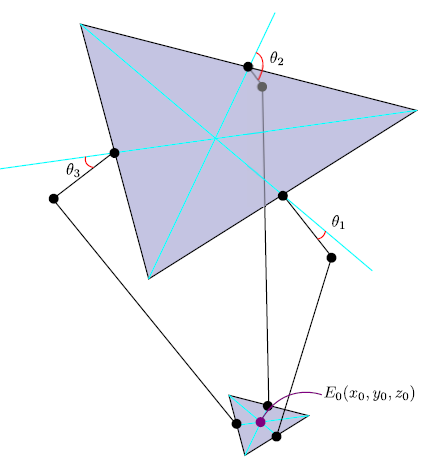
\includegraphics[width=0.5\linewidth]{Main/Chapter4/Images4/Metodo_A_Modelacion_Cinematica_Posicion_1.png}
              \caption{Fotografía de un paraguas}
              \label{f:Cap4_Metodo_A_Modelacion_Cinematica_Posicion_1}
        \end{figure}

 

        En la figura \ref{f:Cap4_Metodo_A_Modelacion_Cinematica_Posicion_1} se aprecia las piezas mecánicas básicas de un robot delta, tales como la  base fija, un efector móvil , brazos y antebrazos. En la siguiente tabla muestra la relación entre la numeración en la figura \ref{f:Cap4_Metodo_A_Modelacion_Cinematica_Posicion_1} y su descripción:
        
        \begin{table}[h]
            \centering
            \begin{tabular}{c c}
            \hline
                \textbf{Numero}& \textbf{Descripción} \\ 
            \hline             \hline
             1 & Base fija \\
            \hline
             2 & Brazo \\
            \hline
             3 & Junta esférica \\
            \hline
             4 & Antebrazo\\
            \hline
             5 & Efector final \\
             \hline
             6 & Actuador  \\
             \hline
            \end{tabular}
           \caption{Referencias del dibujo}
           \label{tab:cap4_tabla_1}
        \end{table}

        \newpage
        
        \begin{figure}[htb]
             \centering
             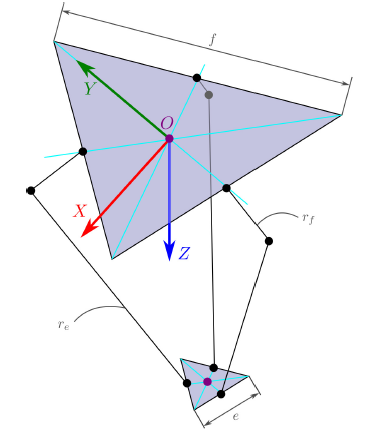
\includegraphics[width=0.6\linewidth]{Main/Chapter4/Images4/Metodo_A_Modelacion_Cinematica_Posicion_2.png}
              \caption{Fotografía de un paraguas}
              \label{f:Cap4_Metodo_A_Modelacion_Cinematica_Posicion_2}
        \end{figure}
        
        En la siguiente tabla se presenta la simbología de los principales parámetros para el desarrollo de la solución cinemática propuesta en este capitulo: 
        
        \begingroup
            \renewcommand{\arraystretch}{1.5}
            \begin{table}[H]
            \centering
            \begin{tabular}{c m{12cm}}
               \hline
               \textbf{Simbología}  & \multicolumn{1}{c|}{\textbf{Descripción}}  \\\hline\hline
               $r_{f}$  & Longitud del brazo                                    \\\hline
               $r_{e}$  & Longitud del antebrazo                                \\\hline               
               $f$  & Lado de base fija                                         \\\hline
               $e$  & Lado del efector                                          \\\hline
               $\theta_{i}$  & Ángulo del actuador i    \\\hline
               $F_{i}$  & Coordenadas de la posición del actuador i=1,2,3.    \\\hline
               $E_{i}$  & Coordenadas de las juntas esféricas que unen el antebrazo con el efector (punto medio del lado
               del triangulo que forma el efector) i=1,2,3.    \\\hline
               $E_{0}(x_{0},y_{0},z_{0})$  & Coordenadas del centroide del efector   \\\hline               
            \end{tabular}
            \caption{Referencias del dibujo}
            \label{tab:cap4_tabla_2}
        \end{table}
        \endgroup
        
        
        
        
        \newpage

    
        \subsubsection{Cinemática directa} \label{ma_cd}
        El fin de la cinemática directa es hallar la posición del efector final del robot delta dada una configuración articular, en este caso la de los actuadores.

        \begin{equation}
            \left({\theta }_1,{\theta }_2,{\theta }_3\right)\ \to E_0(x_0,y_0,z_0)\
        \end{equation}

        \begin{figure}[htb]
             \centering
             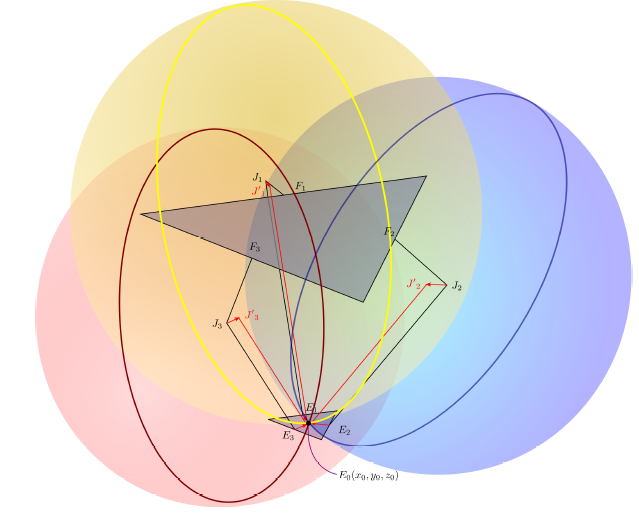
\includegraphics[width=0.8\linewidth]{Main/Chapter4/Images4/Metodo_A_Modelacion_Cinematica_Posicion_3.png}
              \caption{Fotografía de un paraguas}
              \label{f:Cap4_Metodo_A_Modelacion_Cinematica_Posicion_3}
        \end{figure}
        
        Las posiciones en el espacio de los brazos del robot delta ya están definidos gracias a que se conoce los ángulos de los actuadores $({\theta }_1,{\theta }_2,{\theta }_3)$ y la longitud de los brazos $r_f$. 
        
        Por otro lado, de los antebrazos solo se conoce la posición de la junta esférica $J_i$ que los une con los brazos. Como resultado del incompleto conocimiento espacial de esta pieza, la posición y orientación de cada antebrazo está restringida por una esfera con centro en la junta esférica $J_i$, con radio equivalente al largo del antebrazo $r_e$. 
        
        Para finalizar se realiza una traslación de las esferas mencionadas anteriormente para obtener las coordenadas del centroide del efector final $E_0$. Esta translación produce 3 nuevas esferas, con nuevos centros y de radio equivalente al largo del antebrazo $r_e$. Las nuevas esferas se intersecan en el centroide del efector $E_0$ .Como último paso, para calcular las coordenadas del punto $E_0(x_0,y_0,z_0)$ se realiza un sistema de ecuaciones no lineal con 3 restricciones (esferas que contienen los antebrazos) y 3 incógnitas (coordenadas $(x_0,y_0,z_0)$ del efector final) .

        \newpage
        
        Los 3 centros y radios de las nuevas esferas que se intersecan en el centroide del efector $E_0(x_0,y_0,z_0)$ son:
        
    \vspace{-1em}

        \begin{center}
        \renewcommand{\arraystretch}{2.5}
        
            \begin{table}[H]
            \centering
            \begin{tabular}{p{1.4cm} c c } 
                 \hline
                 \textbf{Centros}  &  \textbf{Centros esferas}  & \textbf{Radio} \\ [0.1ex] 
                 \hline\hline
                         $\left(x_1,y_1,z_1\right)$ &
                         ${J^'}_1\left(0,\left[-\frac{f-e}{2\sqrt{3}}-r_f{\mathrm{cos} \left({\theta }_1\right)\ }\right],-r_f{\mathrm{sin}\mathrm{n} \left({\theta }_1\right)\ }\right)$ & 
                                                 $r_e$ \\ 
                \hline
                          $\left(x_2,y_2,z_2\right)$ & ${J^'}_2(\left[\frac{f-e}{2\sqrt{3}}+r_f{\mathrm{cos} \left({\theta }_2\right)\ }\right]\mathrm{cos}\mathrm{}(30{}^\circ ),\left[\frac{f-e}{2\sqrt{3}}+r_f{\mathrm{cos} \left({\theta }_2\right)\ }\right]\mathrm{sin}\mathrm{}(30{}^\circ ),-r_f{\mathrm{sin} \left({\theta }_2\right)\ })$ & $r_e$ \\
                \hline
                           $\left(x_3,y_3,z_3\right)$ & ${J^'}_3(-\left[\frac{f-e}{2\sqrt{3}}+r_f{\mathrm{cos} \left({\theta }_3\right)\ }\right]\mathrm{cos}\mathrm{}(30{}^\circ ),\left[\frac{f-e}{2\sqrt{3}}+r_f{\mathrm{cos} \left({\theta }_3\right)\ }\right]\mathrm{sin}\mathrm{}(30{}^\circ ),-r_f{\mathrm{sin} \left({\theta }_3\right)\ })$ & $r_e$ \\ [1ex] 
                 \hline
            \end{tabular}
            \caption{Referencias del dibujo}
            \label{tab:cap4_tabla_3}
            \end{table}
        \end{center}
        
    \vspace{-3.5em}

    Para simplificar las ecuaciones algebraicas de las esferas, se escriben los centros $\left(x_i,y_i,z_i\right)\ ,\ i=1,2,3$
    
        \vspace{-1em}

    
    \begin{equation}
    \left\lbrace
    \begin{array}{ll}
    {\left(x-x_1\right)}^2+{\left(y-y_1\right)}^2\ +{\left(z-z_1\right)}^2=\ {r_e}^2\  \\ 
    {\left(x-x_2\right)}^2+{\left(y-y_2\right)}^2\ +{\left(z-z_2\right)}^2=\ {r_e}^2 \\ 
    {\left(x-x_3\right)}^2+{\left(y-y_3\right)}^2\ +{x\left(z-z_3\right)}^2=\ {r_e}^2
    \end{array}
    \right.
    \label{eq:cap4_eq_2}
    \end{equation}


    Despu\'{e}s de un extenso desarrollo alg\'{e}brico, la soluci\'{o}n del sistema de ecuaciones  (\ref{eq:cap4_eq_2}) es:

    \vspace{-2.5em}

    \begin{align}
    \begin{split}
            E_0\left(x_0,y_0,z_0\right)&={} \left(a_1z+\ b_1,a_2z+\ b_2,\frac{-B-\ \sqrt{\left(B^2\right)-\left(4AC\right)}}{2*A}\right)\\
    \end{split}
    \label{eq:cap4_eq_3}
    \end{align}
    

    Donde:
    \vspace{-1.0em}
        
    \begin{align}
        z={}& \frac{-B-\ \sqrt{\left(B^2\right)-\left(4AC\right)}}{2A}
        \label{eq:cap4_eq_4} \\
        A={}& {a_1}^2+{a_2}^2+1
        \label{eq:cap4_eq_5} \\
        B={}&  2\left(a_1(b_1-x_1)+a_2(b_2-y_1)-z_1\right)
        \label{eq:cap4_eq_6} \\
        C={}& ({(b_1-x_1)}^2+{(b_2-y_1)}^2+{z_1}^2- {r_e}^2) 
        \label{eq:cap4_eq_7} \\
        a_1={}& \frac{\left(z_2-z_1\right)\left(y_3-y_1\right)-\left(z_3-z_1\right)\left(y_2-y_1\right)}{d} 
        \label{eq:cap4_eq_8} \\
        b_1={}& \left(\frac{1}{2*(-d)}\right)*\left(\left(w_2 - w_1\right)\left(y_3-y_1\right)-\left(w_3 - w_1\right)\left(y_2-y_1\right)\right)
        \label{eq:cap4_eq_9} \\
        a_2={}& \frac{-1}{d}*\left[\left(z_2-z_1\right)x_3-(z_3-z_1)x_2+(z_3-z_2)x_1\right]
        \label{eq:cap4_eq_10} \\
        b_2={}& \frac{1}{2d}*[\left(w_2-w_1\right)x_3-\left(w_3-w_1\right)x_2+\left(w_3-w_2)x_1\right]
        \label{eq:cap4_eq_11} \\
        d={}& \left(y_2- y_1\right)x_3-\left(y_3-y_1\right)x_2- \left(y_2-y_3\right)x_1
        \label{eq:cap4_eq_12} \\
        w_i={}& {x_i}^2+{y_i}^2 +{z_i}^2
        \label{eq:cap4_eq_13} 
    \end{align}

         \newpage


        \subsubsection{Cinemática inversa} \label{ma_ci}
        El objetivo de la cinemática inversa es hallar la posición de los actuadores en el espacio articular dada la posición del centroide del efector final.
        
        \begin{equation}
            E_0(x_0,y_0,z_0)\ \to \left({\theta }_1,{\theta }_2,{\theta }_3\right)
        \end{equation}
        
        
        \begin{figure}[htb]
             \centering
             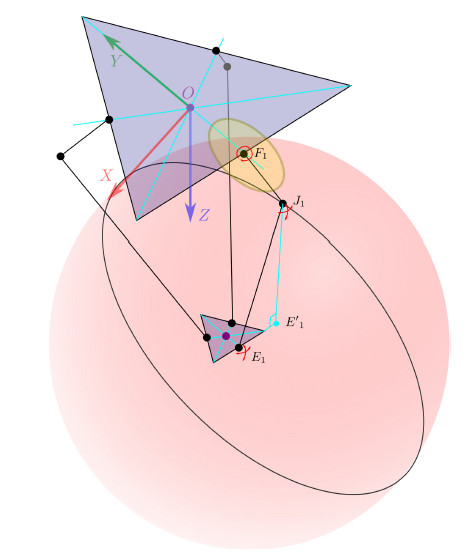
\includegraphics[width=0.35\linewidth]{Main/Chapter4/Images4/Metodo_A_Modelacion_Cinematica_Posicion_4.png}
              \caption{Fotografía de un paraguas}
              \label{f:Cap4_Metodo_A_Modelacion_Cinematica_Posicion_4}
        \end{figure}
        
         Se tiene la informaci\'{o}n de las coordenadas de las juntas esf\'{e}ricas $E_i$ a causa de que se sabe la posici\'{o}n centroide del efector final $E_0(x_0,y_0,z_0)$ y que cada lado del tri\'{a}ngulo formado por la base fija son paralelos a los lados del triangulo formado por el efector, es decir, tanto la orientaci\'{o}n como la inclinaci\'{o}n entre la base fija y el efector son iguales.  

        En relaci\'{o}n con los antebrazos, solo se conoce el punto $E_i$ , que coincide con las posiciones de cada junta esf\'{e}rica unida al efector. Esto trae como consecuencia que cada antebrazo esta restringido por esferas con centros en las juntas esf\'{e}ricas $E_i$ con radio equivalente al largo del antebrazo $r_e$.
    
        Acerca de los brazos solo se tiene conocimiento de los puntos $F_i$, que son la posici\'{o}n de cada actuador. Los actuadores son juntas revolutas y restringen le movimiento de cada brazo en planos. La configuraci\'{o}n espacial de estos planos para cada cadena cinem\'{a}tica es determinada por los puntos $F_i$ ,$O$ (origen) y el plano de la que contiene la base fija. El plano que contiene la base fija es perpendicular a los planos que restringen el movimiento de los brazos. En consecuencia, la posici\'{o}n de los puntos extremos de cada brazo, es decir, los puntos $J_i$ (junta esf\'{e}rica), est\'{a}n restringidos por circunferencias como se muestra en la ilustracion \ref{f:Cap4_Metodo_A_Modelacion_Cinematica_Posicion_3} .

        Para finalizar, se calcula la intersecci\'{o}n entre las circunferencias para cada cadena cinem\'{a}tica, en otras palabras, los puntos  $J_i$ . Una vez obtenida la posici\'{o}n de las 3 juntas $J_i$, con algebra simple se calculan $\left({\theta }_1,{\theta }_2,{\theta }_3\right)$.
        
                \newpage


        En el caso del actuador  $i=1$ , los centros de las circunferencias que intersección la junta esf\'{e}rica $J_1$ son:
        
        \begin{center}
        \renewcommand{\arraystretch}{2.5}
        
            \begin{table}[H]
            \centering
            \begin{tabular}{p{1.4cm} c c } 
                 \hline
                 \textbf{Centros}  &  \textbf{Centros esferas}  & \textbf{Radio} \\ [0.1ex] 
                 \hline\hline
                         $\left(y_1,z_1\right)$ &
                        $F_1\left(y_{F_1}\,z_{F_1}\right)=\left(-\frac{f}{2\sqrt{3}},0\right)$\textit{} & 
                                                 $r_f$  \\ 
                \hline
                          $(y_2,z_2)$&
                          ${E^'}_{1}$ $(y_{{E^'}_1}$ $z_{{E^'}_1}$ $)=(y_0-\frac{e}{2\sqrt{3}},z_0)$ &
                          $r_2=\sqrt{{r_e}^2-{x_o}^2}$ \\
                \hline
            \end{tabular}
            \caption{Referencias del dibujo}
            \label{tab:cap4_tabla_4}
            \end{table}
        \end{center}
    \vspace{-2.5em}
        
Las ecuaciones cartesianas de las dos circunferencias quedan representadas en términos de  $y_{1},z_{1},r_{f},r_{f},~y_{2},z_{2},\sqrt[]{r_{e}^{2}-x_{o}^{2}}$ para simplificar la escritura de los cálculos:

    \begin{equation}
    \left\lbrace
    \begin{array}{ll}
    \left( y-y_{1} \right) ^{2} + \left( z-z_{1} \right) ^{2}= r_{f}^{2}~\\
    \left( y-y_{2} \right) ^{2} + \left( z-z_{2} \right) ^{2}= r_{e}^{2}-x_{o}^{2}\\ 
    \end{array}
    \right.
    \label{eq:cap4_eq_15}
    \end{equation}

La solución del sistema de ecuaciones (\ref{eq:cap4_eq_15}) es:

    \begin{equation}
    J_{1}= \left( x_{J_{1}},y_{J_{1}},z_{J_{1}} \right) = \left( 0,y,a+by \right)
    \label{eq:cap4_eq_16}
    \end{equation}

    Donde:

    \begin{equation}
        y=\frac{\left( y_{1}-ab \right) -\sqrt[]{ \left[  -\left( a+by_{1} \right) ^{2}+ \left( b^{2}+1 \right) r_{f}^{2} \right] }}{ \left( b^{2}+1 \right) }
    \label{eq:cap4_eq_17}
    \end{equation}

    \begin{equation}
        b=\frac{ \left( y_{1}-y_{2} \right) }{z_{2}}~ 
    \label{eq:cap4_eq_18}
    \end{equation}
    
    \begin{equation}
        a= \frac{x_{o}^{2}+y_{2}^{2}+z_{0}^{2}+r_{f}^{2}- r_{e}^{2}~-y_{1}^{2}}{2z_{0}} 
    \label{eq:cap4_eq_19}
    \end{equation}

                \newpage

En último lugar, se determina el ángulo \( ~ \theta _{1} \)  por medio del triángulo rectángulo formado en el brazo y la proyección del mismo en el plano XY:

    \begin{equation}
        \theta _{1}=\arctan  \left( ~\frac{z_{J_{1}}}{y_{F_{1}}-y_{J_{1}}} \right)  
        \label{eq:cap4_eq_20}
    \end{equation}
    
    Donde:  \( y_{F_{1}}= - \frac{f}{2~\sqrt[]{3}} \)

    
        \begin{figure}[htb]
             \centering
             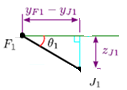
\includegraphics[width=0.25\linewidth]{Main/Chapter4/Images4/Metodo_A_Modelacion_Cinematica_Posicion_5.png}
              \caption{Fotografía de un paraguas}
              \label{f:Cap4_Metodo_A_Modelacion_Cinematica_Posicion_5}
        \end{figure}




Se emplea el mismo procedimiento anterior para encontrar los ángulos  \(  \theta _{2} \)  y  \(  \theta _{3} \)  por medio de matrices de rotación, con un ángulo de rotación de 120$ ^{\circ} $  para la cadena cinemática con el actuador 2 y de 240$ ^{\circ} $  para la cadena cinemática con el actuador 3. Estas matrices giran el sistema de referencia local en 120$ ^{\circ} $  y 240$ ^{\circ} $ . 

        \begin{figure}[htb]
             \centering
             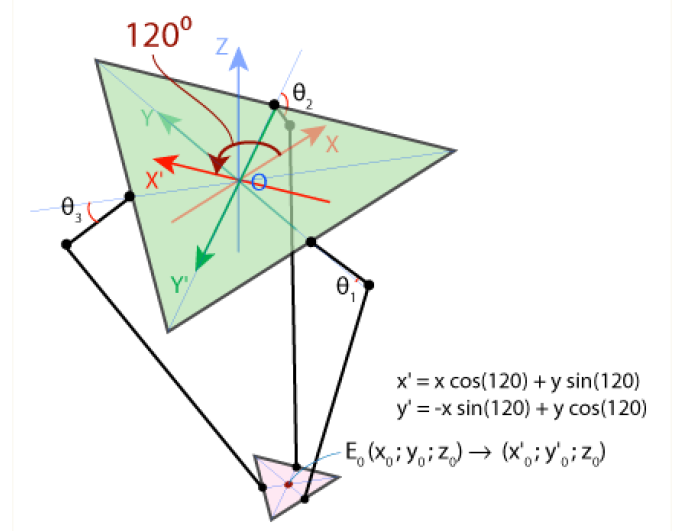
\includegraphics[width=0.8\linewidth]{Main/Chapter4/Images4/Metodo_A_Modelacion_Cinematica_Posicion_6.png}
              \caption{Fotografía de un paraguas}
              \label{f:Cap4_Metodo_A_Modelacion_Cinematica_Posicion_6}
        \end{figure}

        \newpage

    \subsection{Modelación cinemática de la velocidad}\label{ma_cvel}
        En esta sección, se da a conocer un método para calcular la matriz jacobiana y su estrecha relación con las singularidades de un robot paralelo tipo delta. Se implementan las ideas extraídas del paper \cite{Hsu_modelling_ai}
    
        \subsubsection{Nomenclatura de Parámetros Geométricos y Sistema deReferencia Loca}
        
        En la ilustración \ref{f:Cap4_Metodo_A_Modelacion_Cinematica_Posicion_7} se pueden visualizar 3 cadenas cinemáticas las cuales se componen de 4 partes mecánicas: la base fija, los brazos accionados, las barras seguidoras y la plataforma móvil.
        
        \begin{figure}[htb]
             \centering
             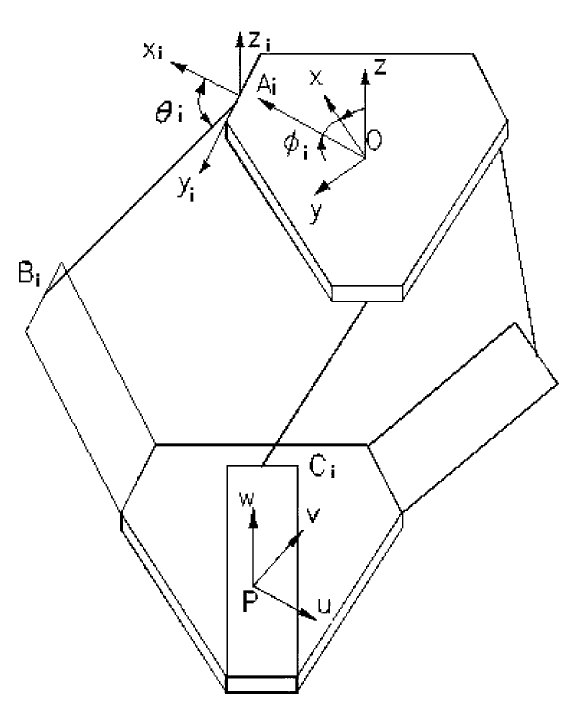
\includegraphics[width=0.45\linewidth]{Main/Chapter4/Images4/Metodo_A_Modelacion_Cinematica_Posicion_7.png}
              \caption{Fotografía de un paraguas}
              \label{f:Cap4_Metodo_A_Modelacion_Cinematica_Posicion_7}
        \end{figure}
        
        
        En la tabla \ref{tab:cap4_tabla_5} muestra la relación entre la numeración en la figura anterior y su descripción:
        
        \begin{table}[h]
            \centering
            \begin{tabular}{c c}
            \hline
                \textbf{Numero}& \textbf{Descripción} \\ 
            \hline             \hline
             1 & plataforma móvil \\
            \hline
             2 & barras seguidoras \\
            \hline
             3 & brazos accionados \\
            \hline
             4 & base fija\\
            \hline
             5 & Juntas universales \\
             \hline
            \end{tabular}
           \caption{Referencias del dibujo}
           \label{tab:cap4_tabla_5}
        \end{table}
      
    \newpage

      En la tabla \ref{tab:cap4_tabla_6} se presenta la simbologia de las principales longitudes para el desarrollo de la solución cinematica propuesta en este capitulo:

        \begingroup
            \renewcommand{\arraystretch}{1.5}
            \begin{table}[H]
            \centering
            \begin{tabular}{c m{12cm}}
               \hline
               \textbf{Simbología}  & \multicolumn{1}{c}{\textbf{Descripción}}  \\
               \hline           \hline            
             $a$ & Longitud de los brazos accionados \\
            \hline
             $b$ & Longitud de las barras seguidoras \\
            \hline
             $r$ & Longitud desde el centro de la base fija a un actuador i \\
            \hline
             $h$ & Longitud del centro de la plataforma móvil a una junta universal unida a él.\\
            \hline
            \end{tabular}
            \caption{Referencias del dibujo}
           \label{tab:cap4_tabla_6}
        \end{table}
        \endgroup        

    En la tabla \ref{tab:cap4_tabla_7} se presenta la simbologia de los principales puntos para el desarrollo de la solucion cinematica propuesta en este capitulo: 
    
        \begingroup
            \renewcommand{\arraystretch}{1.5}
            \begin{table}[H]
            \centering
            \begin{tabular}{c m{12cm}}
               \hline
               \textbf{Simbología}  & \multicolumn{1}{c}{\textbf{Descripción}}  \\\hline
            \hline            
             $A_{i}$ & Punto que representa la posición de actuador i \\
            \hline
             $ B_{i}$ & Punto que representa la posición de las juntas universales que unen los brazos accionados y las barras seguidoras \\
            \hline
             $C_{i}$ & Punto que representa la posición de las juntas universales que unen las barras seguidoras con la plataforma móvil \\
            \hline
             $P$ & Punto que representa el centro de la plataforma móvil.\\
            \hline
            \end{tabular}
            \caption{Referencias del dibujo}
           \label{tab:cap4_tabla_7}
        \end{table}
        \endgroup
    
    En la tabla \ref{tab:cap4_tabla_8} se presenta la simbologia de los principales angulos para el desarrollo de la solucion cinematica propuesta en este capitulo: 
    
        \begingroup
            \renewcommand{\arraystretch}{1.5}
            \begin{table}[H]
            \centering
            \begin{tabular}{c m{12cm}}
               \hline
               \textbf{Simbología}  & \multicolumn{1}{c}{\textbf{Descripción}}  \\\hline
            \hline            
             $\phi _{i}$ & Ángulo que representa la posición angular de los 3 actuadores sobre el plano de la base fija $ \{ $ 0$ ^{\circ} $ , 120$ ^{\circ} $ , 240$ ^{\circ} $ $ \} $ \\
            \hline
             $ \theta _{1i}$ & Angulo que representa la posición angular de las barras accionadas respecto al eje que contiene los puntos del origen del sistema de referencia local y A_{i}  \\
            \hline
            \end{tabular}
            \caption{Referencias del dibujo}
           \label{tab:cap4_tabla_8}
        \end{table}
        \endgroup    
    
        \newpage
    
        En la tabla \ref{tab:cap4_tabla_9} se presenta la simbologia de los principales sistemas de referencia para el desarrollo de la solucion cinematica propuesta en este capitulo: 
        
        \begingroup
            \renewcommand{\arraystretch}{1.5}
            \begin{table}[H]
            \centering
            \begin{tabular}{c m{12cm}}
               \hline
               \textbf{Simbología}  & \multicolumn{1}{c}{\textbf{Descripción}}  \\\hline
            \hline            
             $O$ – $xyz$ & Ángulo que representa la posición angular de los 3 actuadores sobre el plano de la base fija $ \{ $ 0$ ^{\circ} $ , 120$ ^{\circ} $ , 240$ ^{\circ} $ $ \} $ \\
            \hline
             $  A_{i}$ – $x_{i}y_{i}z_{i}$ & Angulo que representa la posición angular de las barras accionadas respecto al eje que contiene los puntos del origen del sistema de referencia local y A_{i}  \\
            \hline
            \end{tabular}
            \caption{Referencias del dibujo}
           \label{tab:cap4_tabla_9}
        \end{table}
        \endgroup        
        
    \newpage

        \subsubsection{Vectorización y ángulos de las articulaciones} \label{cap4_angulosinteriores}
        
        La ilustracion \ref{f:Cap4_Metodo_A_Modelacion_Cinematica_Posicion_8} define los ángulos de articulación asociados con la extremidad  \( i \) .  \(  \theta _{2i} \)  se define desde la línea extendida de  \( \overrightarrow{A_{i}B_{i}} \)  hasta la línea definida por la intersección del plano del paralelogramo y el plano  \( x_{i}-z_{i} \)  y  \(  \theta _{3i} \)  se mide desde la dirección  \( y_{i} \)  hasta  \( \overrightarrow{B_{i}C_{i}} \) .
        
        \begin{figure}[htb]
             \centering
             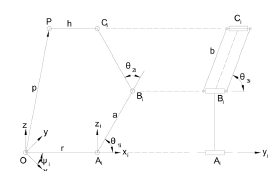
\includegraphics[width=0.8\linewidth]{Main/Chapter4/Images4/Metodo_A_Modelacion_Cinematica_Posicion_8.png}
              \caption{Fotografía de un paraguas}
              \label{f:Cap4_Metodo_A_Modelacion_Cinematica_Posicion_8}
        \end{figure}
        
        
        En la tabla \ref{tab:cap4_tabla_10} se presenta las descripciones de los vectores mostrados \colorbox{Yellow}{en la ilustración de arriba:}
        
        \begingroup
            \renewcommand{\arraystretch}{1.5}
            \begin{table}[H]
            \centering
            \begin{tabular}{c m{12cm}}
               \hline
               \textbf{Simbología}  & \multicolumn{1}{c}{\textbf{Descripción}}  \\\hline
            \hline            
             \overrightarrow{A_{i}B_{i}} & Vector que representa el brazo accionado i \\
            \hline
             \overrightarrow{B_{i}C_{i}} & Vector que representa la barra seguidora i.  \\
            \hline
             \overrightarrow{OP} & Vector que representa el centro de la plataforma móvil.  \\
            \hline
             \overrightarrow{PC_{i}} & Vector que representa la distancia entre el centro de la plataforma móvil y una junta universal unidad a la cadena cinemática i.  \\
            \hline
             \overrightarrow{OA_{i}} & Vector que representa la posición de los actuadores respecto al origen O.  \\
            \hline
            \end{tabular}
            \caption{Referencias del dibujo}
           \label{tab:cap4_tabla_10}
        \end{table}
        \endgroup      
        

      Se puede escribir una ecuación de cierre de bucle para cada extremidad vectorialmente:  
        
    \begin{equation}
    \overrightarrow{A_{i}B_{i}}+ \overrightarrow{B_{i}C_{i}}~~ =\overrightarrow{OP}~ +\overrightarrow{~PC_{i}} -\overrightarrow{OA_{i}~} 
    \label{eq:cap4_eq_21}
    \end{equation}
    
            \newpage

    
    Reescribiendo la ecuacion (\ref{eq:cap4_eq_21}) en el marco de coordenadas $A_{i} – x_{i} y_{i} z_{i}$  conduce a la siguiente representación matricial:   

    \begin{equation}
         a \left[ \begin{matrix}
        cos~ \theta _{1i}\\
        0\\
        sin~ \theta _{1i}\\
        \end{matrix}
         \right] +b \left[ \begin{matrix}
        sin~ \theta _{3i} cos⁡ \left(  \theta _{1i}+ \theta _{2i} \right) \\
        cos~ \theta _{3i}\\
        sin~ \theta _{3i}sin \left(  \theta _{1i}+ \theta _{2i} \right) \\
        \end{matrix}
         \right] = \left[ \begin{matrix}
        \cos  \phi _{i}  &  \sin  \phi _{i}  &  0\\
        -sin \phi _{i}  &  \cos  \phi _{i}  &  0\\
        0  &  0  &  1\\
        \end{matrix}
         \right]  \left[ \begin{matrix}
        p_{x}\\
        p_{y}\\
        p_{z}\\
        \end{matrix}
         \right] +  \left[ \begin{matrix}
        h\\
        0\\
        0\\
        \end{matrix}
         \right] - \left[ \begin{matrix}
        r\\
        0\\
        0\\
        \end{matrix}
         \right] ~= \left[ \begin{matrix}
        c_{xi}\\
        c_{yi}\\
        c_{zi}\\
        \end{matrix}
         \right] ~
        \label{eq:cap4_eq_22}
    \end{equation}    
    
    Donde la posición del punto $C_{i} (c_{xi},c_{yi},c_{zi})$ esta en relación con el marco de coordenadas $A_{i}$ – $x_{i} y_{i} z_{i}$.
    
    Realizando algebra en la ecuación anterior se puede determinar los ángulos $\theta_{2i}$ y $\theta_{3i}$ con las siguientes ecuaciones: 
    
    \begin{equation}
       \theta _{3i}= \cos ^{-1}\frac{c_{yi}}{b} 
        \label{eq:cap4_eq_23}
    \end{equation}
     
    \begin{equation}
    \theta _{2i}=\cos ^{-1} \left( \frac{c_{xi}^{2}+c_{yi}^{2}+c_{zi}^{2}-a^{2}-b^{2}~}{2ab sin~ \theta _{3i}} \right) 
     \label{eq:cap4_eq_24}
    \end{equation}
    
    
    Con $\theta _{3i}$ y $\theta_{2i}$ determinados, solo queda un par de ecuaciones con $\theta_{1i}$ como la única incógnita que se deriva de la ecuacion (\ref{eq:cap4_eq_22}). Por lo tanto, es posible obtener  $\theta_{1i}$.

    
        \newpage

        \subsubsection{Jacobiano}\label{ma_jac}
        
        La matriz jacobiana tradicional proporciona una transformación de la velocidad del efector final en el espacio cartesiano a las velocidades articulares accionadas.
        
        \begin{figure}[htb]
             \centering
             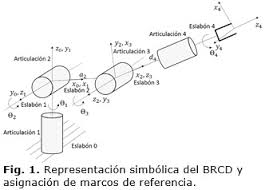
\includegraphics[width=0.5\linewidth]{Main/Chapter4/Images4/Metodo_A_Modelacion_Cinematica_Posicion_10.png}
              \caption{Fotografía de un paraguas}
              \label{f:Cap4_Metodo_A_Modelacion_Cinematica_Posicion_10}
        \end{figure}
        
        Con referencia a la ilustracion \ref{f:Cap4_Metodo_A_Modelacion_Cinematica_Posicion_10}, una ecuación de cierre de bucle para una extremidad i en marco de coordenadas  \( A_{i} \) – \( x_{i}y_{i}z_{i} \) se puede escribir como:
        
        \begin{equation}
             \overrightarrow{OP}+\overrightarrow{~PC_{i}} =\overrightarrow{OA_{i}}+\overrightarrow{A_{i}B_{i}}+\overrightarrow{B_{i}C_{i}}  
         \label{eq:cap4_eq_25}
        \end{equation}

        Al diferenciar vectorialmente la ecuación (\ref{eq:cap4_eq_25}) con respecto a el tiempo y separando las componentes de velocidad de la plataforma móvil de las velocidades angulares de los actuadores se llega a la siguiente expresión:
        
        \begin{equation}
            J_{x}v_{p}=J_{ \theta }\dot{ \theta } 
            \label{eq:cap4_eq_26}
        \end{equation}
        
        La expresion matricial de la ecuacion (\ref{eq:cap4_eq_26}) es:
        
        \begin{equation}
                \left[ \begin{matrix}
                J_{1x}  &  J_{1y}  &  J_{1z}\\
                J_{2x}  &  J_{2y}  &  J_{2z}\\
                J_{3x}  &  J_{3y}  &  J_{3z}\\
                \end{matrix}
                 \right]  \left[ \begin{matrix}
                v_{px}\\
                v_{py}\\
                v_{pz}\\
                \end{matrix}
                 \right] = \left[ \begin{matrix}
                J_{1 \theta }~  &  0  &  0\\
                0  &  J_{2 \theta }~~  &  0\\
                0  &  0  &  J_{3 \theta }~\\
                \end{matrix}
                 \right]  \left[ \begin{matrix}
                \dot{ \theta _{11}}~\\
                \dot{ \theta _{12}}\\
                \dot{ \theta _{13}}~\\
                \end{matrix}
                 \right]
                \label{eq:cap4_eq_27}
        \end{equation}
        
    Donde: 
    
    \begin{equation}
        J_{ix}=\cos  \left(  \theta _{1i}+ \theta _{2i} \right) sin~ \theta _{3i}\cos  \phi _{i}-cos  \theta _{3i}\sin  \phi _{i}~
        \label{eq:cap4_eq_28}
    \end{equation}
    \vspace{-3.5em}

    \begin{equation}
        J_{iy}=\cos  \left(  \theta _{1i}+ \theta _{2i} \right) sin~ \theta _{3i}\sin  \phi _{i}+ cos  \theta _{3i}\cos  \phi _{i}~ 
        \label{eq:cap4_eq_29}
    \end{equation}
    \vspace{-3.5em}

    \begin{equation}
          J_{iz}=sin \left(  \theta _{1i}+ \theta _{2i} \right) sin~ \theta _{3i}~  
          \label{eq:cap4_eq_30}
    \end{equation}
    \vspace{-3.5em}

    \begin{equation}
         J_{i \theta }=a~\sin  \theta _{2i}~sin~ \theta _{3i}
         \label{eq:cap4_eq_31}
    \end{equation}
         \vspace{-3.5em}
   
            \newpage
    
    Manipulando algebraicamente la ecuación (\ref{eq:cap4_eq_26}):
    
     \begin{equation}
        v_{p}=J\dot{ \theta }
        \label{eq:cap4_eq_32}
    \end{equation}   
    
    Finalmente, el jacobiano es $J$ y representa el cambio de las posiciones en el espacio cartesiano de la plataforma móvil respecto al cambio de los ángulos en el espacio articular de los actuadores:
        
    \begin{equation}
          ~~J= \left[ \begin{matrix}
            \frac{ \partial x}{ \partial  \theta _{1}}  &  \frac{ \partial x}{ \partial  \theta _{2}}  &  \frac{ \partial x}{ \partial  \theta _{3}}\\
            \frac{ \partial y}{ \partial  \theta _{1}}  &  \frac{ \partial y}{ \partial  \theta _{2}}  &  \frac{ \partial y}{ \partial  \theta _{3}}\\
            \frac{ \partial z}{ \partial  \theta _{1}}  &  \frac{ \partial z}{ \partial  \theta _{2}}  &  \frac{ \partial z}{ \partial  \theta _{3}}\\
        \end{matrix}
        \right]   
         \label{eq:cap4_eq_33}
    \end{equation}\    
        
        
     Donde: \par

       $J=J_{x}^{-1}J_{ \theta }$  es el jacobiano del robot delta

        $v_{p}= \left[ v_{px},v_{py},v_{pz} \right] ^{T}$ es la velocidad del del punto  $p$ en la plataforma móvil

        $\dot{ \theta }= \left[ \dot{ \theta _{11}},\dot{ \theta _{12}},\dot{ \theta _{13}}  \right] ^{T}$  es la velocidad angular de los actuadores
        
        \newpage

        
        \subsubsection{Singularidades}\label{CAP4_SINGULARIDAD}
        
        Se debe tener especial cuidado en el diseño de estos manipuladores paralelos para evitar singularidades. Cuando un manipulador está en una posición singular, la matriz jacobiana también es singular. En el caso de los manipuladores paralelos conviene trabajar con un jacobiano de dos partes, matriz jacobiana inversa   $J_{ \theta }$  y la directa  $ J_{x} $ . La ventaja es que un jacobiano bipartito permite, de forma natural, la identificación y clasificación de varios tipos de singularidades. Una de las formas de analizar las singularidades es igualando el determinante de la matriz jacobiana igual a cero y extraer varias posturas indeseables robot delta. Desde la ecuación  (\ref{eq:cap4_eq_26}) se puede observar y clasificar la singularidad en 3 situaciones:
        
        \begin{figure}[htb]
         \centering
          \subfloat[Gatito]{
         \label{f:Cap4_Metodo_A_Modelacion_Cinematica_Posicion_9a}
            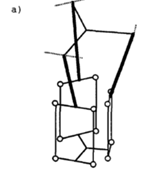
\includegraphics[width=0.3\textwidth]{Main/Chapter4/Images4/Metodo_A_Modelacion_Cinematica_Posicion_9a.png}}
          \subfloat[Tigre]{
         \label{f:Cap4_Metodo_A_Modelacion_Cinematica_Posicion_9b}
            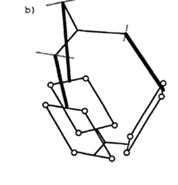
\includegraphics[width=0.3\textwidth]{Main/Chapter4/Images4/Metodo_A_Modelacion_Cinematica_Posicion_9b.png}}
          \subfloat[Conejo]{
         \label{f:Cap4_Metodo_A_Modelacion_Cinematica_Posicion_9c}
            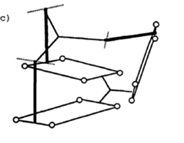
\includegraphics[width=0.3\textwidth]{Main/Chapter4/Images4/Metodo_A_Modelacion_Cinematica_Posicion_9c.png}}
         \caption{Múltiples imágenes}
         \label{f:Cap4_Metodo_A_Modelacion_Cinematica_Posicion_9}
        \end{figure}
        
        \begin{itemize}
	        \item {\fontsize{10pt}{12.0pt}\selectfont Cuando  $\det  \left( J_{ \theta } \right) =0$ . Esto significa que  $\theta _{2i}=0$  o  $\pi$ , o \   $\theta _{3i}=0$ o  $\pi$  , para  \( i = \{ 1,2 ,3 \}  \) . En esta situación los tres pares de barras seguidoras son paralelos. Por tanto, la plataforma móvil tiene tres grados de libertad y se mueve a lo largo de una superficie esférica y gira sobre el eje perpendicular a la plataforma móvil (ilustracion \ref{f:Cap4_Metodo_A_Modelacion_Cinematica_Posicion_9a}) .Al mismo tiempo esta configuración representa el límite del espacio de trabajo, es decir, los puntos más lejanos que puede alcanzar el robot. }

	        \item {\fontsize{10pt}{12.0pt}\selectfont Cuando  $\det  \left( J_{x} \right) =0 $ . Esto significa que    $ \theta _{1i}+  \theta _{2i}=0$  o  $\pi$ , o $\theta _{3i}=0$  o  $ \pi $   , para  \( i = \{ 1,2 ,3 \}  \) . En esta situación dos pares de barras seguidoras son paralelas. Los la plataforma móvil tiene un grado de libertad; es decir, la plataforma móvil se mueve en una sola dirección (ilustracion \ref{f:Cap4_Metodo_A_Modelacion_Cinematica_Posicion_9b}).}

	        \item {\fontsize{10pt}{12.0pt}\selectfont Cuando $ \det  \left( J_{ \theta } \right) =0 $  y $ \det  \left( J_{x} \right) =0 $. Esta situación ocurre cuando  $  \theta _{3i}=0$ o  $ \pi  $  , para  \( i = \{ 1,2 ,3 \}  \) . En esta situación dos pares de barras seguidoras están en el mismo plano o dos planos paralelos. La plataforma móvil tiene un grado de libertad; es decir, la plataforma móvil gira sobre el eje horizontal solamente (ilustracion \ref{f:Cap4_Metodo_A_Modelacion_Cinematica_Posicion_9c})}
\end{itemize}

    
    \newpage
    
    \subsection{Modelación Cinematica de Aceleracion}

    En esta sección se presentan las ecuaciones para determinar la aceleración angular de los actuadores del robot delta. La aceleración se determina derivando matricial mente la ecuación (\ref{eq:cap4_eq_26}) de la sección \ref{ma_cvel} modelacion cinemática de velocidad para el método A.

    \vspace{-2.5em}

    \begin{align}
    \begin{split}
          \ddot{ \theta }=J_{ \theta }^{-1}\ast \left[ \dot{J}_{x}v_{p}+J_{x}a_{p}-\dot{J}_{ \theta }\dot{ \theta } \right] 
    \end{split}
    \label{eq:cap4_eq_34}
    \end{align}
    
    
    Las matrices en la ecuacion (\ref{eq:cap4_eq_34}) son: 
        \vspace{-0.5em}
    \begin{multline}
            \left[ \begin{matrix}
        \ddot{ \theta }_{11}~\\
        \ddot{ \theta }_{12}\\
        \ddot{ \theta }_{13}~\\
        \end{matrix}\right] = \left[ \begin{matrix}
        J_{1 \theta }~  &  0  &  0\\
        0  &  J_{2 \theta }~~  &  0\\
        0  &  0  &  J_{3 \theta }~\\
        \end{matrix} \right] ^{-1} \\
    \ast         \left[  \left[ \begin{matrix}
        \dot{J}_{1x}  &  \dot{J}_{1y}  &  \dot{J}_{1z}\\
        \dot{J}_{2x}  &  \dot{J}_{2y}  &  \dot{J}_{2z}\\
        \dot{J}_{3x}  &  \dot{J}_{3y}  &  \dot{J}_{3z}\\
        \end{matrix}\right]   \left[ \begin{matrix}
        v_{px}\\
        v_{py}\\
        v_{pz}\\
        \end{matrix}\right]+\left[ \begin{matrix}
        J_{1x}  &  J_{1y}  &  J_{1z}\\
        J_{2x}  &  J_{2y}  &  J_{2z}\\
        J_{3x}  &  J_{3y}  &  J_{3z}\\
        \end{matrix} \right] \left[ \begin{matrix}
        a_{px}\\
        a_{py}\\
        a_{pz}\\
        \end{matrix}\right] - \left[ \begin{matrix}
        \dot{J}_{1 \theta }~  &  0  &  0\\
        0  &  \dot{J}_{2 \theta }~~  &  0\\
        0  &  0  &  \dot{J}_{3 \theta }~\\
        \end{matrix} \right] \left[ \begin{matrix}
        \dot{ \theta _{11}}~\\
        \dot{ \theta _{12}}\\
        \dot{ \theta _{13}}~\\
        \end{matrix} \right]  \right] ~
        \label{eq:cap4_eq_35}
    \end{multline}
    

    Donde:
    \vspace{-1.0em}
    
    
        \begin{align}
        \dot{J}_{ix}={}& A'_{ix}-B'_{ix}
        \label{eq:cap4_eq_36} \\
        A'_{ix}={}& cos \phi _{i}\ast \left[  \left[ -\sin  \left(  \theta _{1i}+ \theta _{2i} \right) \ast \left( \dot{ \theta }_{1i}+\dot{ \theta }_{2i} \right) \ast sin  \theta _{3i} \right]  + \left[ \cos  \left(  \theta _{1i}+ \theta _{2i} \right) \ast cos  \theta _{3i}\ast\dot{ \theta }_{3i} \right]  \right]
        \label{eq:cap4_eq_37} \\
        B'_{ix}={}& sin \phi _{i}\ast \left[ -sin \theta _{3i}\ast\dot{ \theta }_{3i} \right] 
        \label{eq:cap4_eq_38} \\
        \dot{J}_{iy}={}& A'_{iy}+B'_{iy}
        \label{eq:cap4_eq_39} \\
        A'_{iy}={}& sin \phi _{i}\ast \left[  \left[ -sin \left(  \theta _{1i}+ \theta _{2i} \right) \ast \left( \dot{ \theta }_{1i}+\dot{ \theta }_{2i} \right) \ast sin~ \theta _{3i} \right] + \left[ \cos  \left(  \theta _{1i}+ \theta _{2i} \right) \ast cos  \theta _{3i}\ast\dot{ \theta }_{3i} \right]  \right]
        \label{eq:cap4_eq_40} \\
        B'_{iy}={}& cos \phi _{i}\ast \left[ -sin  \theta _{3i}\ast\dot{ \theta }_{3i} \right]
        \label{eq:cap4_eq_41} \\
        \dot{J}_{iz}={}& \left[ \cos  \left(  \theta _{1i}+ \theta _{2i} \right) \ast \left( \dot{ \theta }_{1i}+\dot{ \theta }_{2i} \right) \ast sin  \theta _{3i} \right] + \left[ sin \left(  \theta _{1i}+ \theta _{2i} \right) \ast cos \theta _{3i}\ast \dot{ \theta }_{3i} \right]
        \label{eq:cap4_eq_42} \\
        \dot{J}_{i \theta }={}&a \left[ ~ \left[ \cos  \theta _{2i}\ast\dot{ \theta }_{2i}\ast \sin  \theta _{3i} \right] + \left[ \sin  \theta _{2i}\ast cos \theta _{3i}\ast\dot{ \theta }_{3i} \right]  \right]
        \label{eq:cap4_eq_43}
    \end{align}
        
\newpage

    \begin{align}
        \dot{ \theta }_{3i}={}& \left[ \frac{-1}{\sqrt[]{1- \left( \frac{c_{yi}}{b} \right) ^{2}~}} \right] \ast \left[ \frac{c_{yi}^{'}}{b} \right]
        \label{eq:cap4_eq_44}\\
        c_{yi}^{'}={}& \left[ -sin \phi _{i}\ast v_{px} + cos \phi _{i}\ast v_{py} \right]
        \label{eq:cap4_eq_45}\\
       \dot{ \theta }_{2i}={}& \left[ \frac{-1}{\sqrt[]{1- \left(  K \right) ^{2}~}} \right] \ast \left[ K' \right]
        \label{eq:cap4_eq_46}\\
        K={}& \frac{c_{xi}^{2}+c_{yi}^{2}+c_{zi}^{2}- a^{2}-b^{2}~}{\text{2 ab }sin~ \theta _{3i}}
        \label{eq:cap4_eq_47}\\
       K^{'}={}& \left[ \frac{1}{2ab} \right] \ast \left[ \frac{A_{11}-A_{12}~}{B_{1}} \right]
        \label{eq:cap4_eq_48}\\
        A_{11}={}& \left[ 2c_{xi}c_{xi}^{'}+2c_{yi}c_{yi}^{'}+2c_{zi}c_{zi}^{'} \right] \ast \left[ sin  \theta _{3i} \right]
        \label{eq:cap4_eq_49}\\
        A_{12}={}& \left[ c_{xi}^{2}+c_{yi}^{2}+c_{zi}^{2}- a^{2}-b^{2} \right] \ast \left[ cos~ \theta _{3i}\ast\dot{ \theta }_{3i} \right]
        \label{eq:cap4_eq_50}\\
        B_{1}={}& \left[ \sin  \theta _{3i} \right] ^{2}
        \label{eq:cap4_eq_51}\\
       c_{xi}^{'}={}& cos \phi _{i}\ast v_{px}+~ sin \phi _{i}\ast v_{py}
        \label{eq:cap4_eq_52}\\
       c_{zi}^{'}={}& v_{pz}
        \label{eq:cap4_eq_53}
    \end{align}


         \newpage






    \newpage

    
    \subsection{Modelación dinámica}
            La aplicación directa de las leyes de Newton al movimiento de sistemas de partículas es sustituida por una propuesta más general, un método para encontrar las ecuaciones de movimiento para todos los sistemas dinámicos, desarrollado por el matemático Joseph Louis Lagrange. En el anexo \ref{anexoB} primero se habla de los conceptos básicos hasta llegar a la formulación de Lagrange. Se obtienen las ecuaciones de Lagrange partiendo del principio de D’Alembert.  Toda la información en esta sección es recopilada en la referencia \cite{INTRO_MECANICA_LAGRAGE}. Finalmente se aplican las ecuaciones de Lagrange al robot delta para determinar el torque de cada actuador.

        \subsubsection{Ecuaciones de Lagrange}

        Se dice que las ligaduras holónomas son empleadas en forma explícita cuando no se utilizan para eliminar las coordenadas dependientes, efectuándose la descripción del sistema de partículas dado con la totalidad (dependientes + independientes) de sus coordenadas. Las ecuaciones de Lagrange para sistemas con ligaduras holónomas usadas de forma explícita se representa en la siguiente formula:
        
        \begin{equation}
             \frac{d}{dt} \left( \frac{ \delta L}{ \delta \dot{q}_{j}} \right) -\frac{ \delta L}{ \delta q_{j}}=Q_{j}^{ \left( lig \right) } \left( q_{j} \right) +Q_{j}^{ \left( NU \right) } \left( q_{j} \right)
             \label{eq:cap4_dina_ma_1}
        \end{equation}
        
        Con  $ j=1,2,3, \ldots , \eta =3N $ 

        Donde:
        \begin{equation}
          Q_{j}^{ \left( lig \right) } \left( q_{j} \right) = \sum _{l=1}^{K^{ \left( h \right) }} \lambda _{l}\frac{ \delta f_{l}^{ \left( h \right) }}{ \delta q_{j}}
             \label{eq:cap4_dina_ma_2}
        \end{equation}

         \( L \)  representa el lagrangiana o lagrangiano:\par
        
        
        \begin{equation}
         L \left( q_{j},\dot{q_{j}},t \right) =T \left( q_{j},\dot{q_{j}},t \right) -V \left( q_{j},\dot{q_{j}},t \right) 
             \label{eq:cap4_dina_ma_3}
        \end{equation}


      Las expresiones (\ref{eq:cap4_dina_ma_1}) son las ecuaciones de Lagrange para ligaduras holónomas  $f_{i}^{(h)}$ $( q_{i},t) =0$  cuando son usadas en forma explícita. Representan un conjunto de  $\eta =3N$  ecuaciones para el conjunto completo de coordenadas (dependientes + independientes)  $q_{1},q_{2},q_{3},...,q_{\eta=3N}$. Estas ecuaciones, en conjunto con las  $K^{ \left( h \right) }$ ecuaciones de ligadura dadas por $f_{i}^{(h)}$ $( q_{i},t) =0$  forman un sistema de   $ 3N+~K^{ \left( h \right) } $  ecuaciones para  $ 3N+~K^{ \left( h \right) } $  incógnitas,  $ 3N $  coordenadas  $ q_{j} $ y  $ K^{ \left( h \right) } $ multiplicadores de Lagrange  $ \lambda _{l}$ , quedando así determinado dicho sistema de ecuaciones. Aquí las ligaduras entran en forma explícita en los  $ Q_{j}^{ \left( lig \right) }$ dados por (\ref{eq:cap4_dina_ma_2}), que son fuerzas adicionales que actúan sobre el sistema. Debido a que estas fuerzas están relacionadas con las ligaduras se les da el nombre de fuerzas generalizadas de ligadura, las cuales no realizan trabajo virtual como lo requiere la validez del Principio de D’Alembert.


    \newpage
    
    
     $ Q_{j}^{ \left( NU \right) }$ son llamadas comúnmente fuerzas generalizadas, sin embargo, no solo son fuerzas. Estas dependen de la dimensión de las coordenadas generalizadas  $ q_{j}$ que se utiliza en la ecuación de Lagrange :
    
    \begin{enumerate}
    	\item Si $q_{j}$  es una longitud, entonces $Q_{j}^{ \left( NU \right)}$  es una fuerza.
    	\item Si  $q_{j}$  es un ángulo, entonces  $Q_{j}^{ \left( NU \right) }$  es un torque.
        \item Si  $q_{j}$  es una superficie, entonces  $Q_{j}^{ \left( NU \right) }$ es una tensión.
    	\item Si $q_{j}$ es un volumen, entonces es $Q_{j}^{ \left( NU \right) }$ una presión.
    \end{enumerate}

    \newpage


    \subsubsection{Nomenclatura de Parameros Geométricos y Sistema de Referencia Global}
    
        \begin{figure}[H]
    		    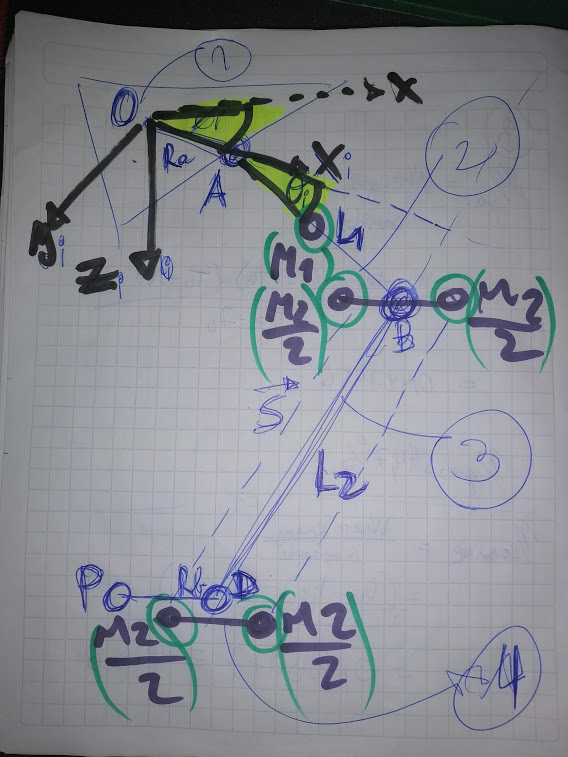
\includegraphics[width=3.43in,height=4.39in]{Main/Chapter4/Images4/ma_dina_1.png}
        \end{figure}

En la ilustración tanto se pueden visualizar 3 cadenas cinemáticas i=1,2,3 las cuales se componen de 4 partes mecánicas: la base fija, brazos, antebrazos y base móvil. La junta que une la base fija con los brazos representan una junta tipo revoluta accionadas por motores. También se muestra la simplificación de masas para resolver la dinámica del robot delta.

En la siguiente tabla muestra la relación entre la numeración en la figura anterior y su descripción:


        \begin{table}[h]
            \centering
            \begin{tabular}{c c}
            \hline
                \textbf{Numero}& \textbf{Descripción} \\ 
            \hline             \hline
             1 & Base fija \\
            \hline
             2 & Brazo \\
            \hline
             3 & Antebazo \\
            \hline
             4 & Base Movil\\
            \hline
            \end{tabular}
           \caption{Referencias del dibujo}
           \label{tab:cap4_tabla_dina_ma_1}
        \end{table}

    \newpage
   
   En la tabla \ref{tab:cap4_tabla_dina_ma_2} se presenta la simbología de los sistema de referencia, magnitudes, puntos y angulos principales para el desarrollo de la dinámica inversa del robot delta:
   
           \begin{table}[h]
            \centering
                \begin{tabular}{c m{11cm}}
            \hline
                \textbf{Simbolo}& \textbf{Descripción} \\ 
            \hline             \hline
             $L_{1}$ &  Longitud brazo\\
            \hline
             $L_{2}$ & Longitud antebrazo \\
            \hline
            $ r_{a}$ &  Radio de circulo inscrito en triangulo de base fija\\
            \hline
             $r_{b}$ & Radio de circulo inscrito en triangulo de base móvil \\
            \hline
            $m_{1}$ & Masa de un brazo posicionada en su centroide \\
            \hline
             $m_{2}$ & Masa de una de las dos barras de los antebrazos, distribuida equitativamente en las extremidades. \\
            \hline
             $A_{i}$ & Punto de unión entre base fija y brazo para la cadena cinematica i \\
            \hline
             $B_{i}$ & Punto de unión entre brazo y antebrazo para la cadena cinematica i \\
            \hline
             $D_{i}$ & Punto de unión entre antebrazo y base móvil para la cadena cinematica i \\
            \hline
             $P$ & Centroide base móvil\\
            \hline
             $\phi _{i}$ & Angulo que representa la posición angular de los 3 actuadores sobre el plano de la base fija en relación al sistema de referencia  –  para la cadena cinemática i. \\
            \hline
             $\theta _{i}$ & Angulo que representa la posición angular de los brazos respecto al eje construido por el punto del origen del sistema de referencia local  y  para la cadena cinemática i.\\
            \hline
             $O –- xyz$ & Sistema de referencia local utilizado para resolver la dinámica del robot delta \\
            \hline
            $A_{i} –- x_{i}y_{i}z_{i}$ & Sistema de referencia con origen coincidente en la junta revoluta que una la base fija con los brazos para la cadena cinemática i \\
            \hline
            \end{tabular}
           \caption{Referencias del dibujo}
           \label{tab:cap4_tabla_dina_ma_2}
        \end{table}
   

    \newpage


    \subsubsection{Dinámica Inversa}
    
        Un paso importante en el proceso de diseño de un robot es comprender el comportamiento del dispositivo mientras se mueve por su espacio de trabajo o al realizar una tarea específica. Este comportamiento se determina mediante el estudio de la dinámica del mecanismo, donde se pueden determinar las fuerzas que actúan sobre los elementos y los pares requeridos por los actuadores. En consecuencia, cada componente debe optimizarse en dimensiones y material para ser utilizado en los procesos de fabricación. Por lo tanto, es esencial buscar cuáles son los enfoques comunes utilizados para calcular la dinámica del robot. Hay tres enfoques: en primer lugar, la formulación de Newton-Euler, que es un método tradicional basado en las leyes de Newton, pero necesita una gran cantidad de ecuaciones, ya que requiere establecer un número n de ecuaciones para cada elemento con el fin de resolver el sistema. Como resultado, es el método más lento en cuanto a eficiencia computacional. En segundo lugar, el trabajo virtual de Principio, que es una derivación del método de Euler y Lagrange utilizando el cálculo de variaciones, se ha utilizado para estudiar la mecánica de los cuerpos deformables. Este enfoque establece que el trabajo total realizado por una fuerza a lo largo de la trayectoria sobre una partícula se puede calcular si esas fuerzas actúan cuando la partícula se mueve del punto A al punto B. Finalmente, la formulación lagrangiana, que se basa en variaciones de cálculo, establece que un sistema dinámico puede expresarse en términos de su energía cinética y potencial conduciendo de manera sencilla a la solución del problema. Además, se considera una buena opción para el control en tiempo real de manipuladores paralelos.
    
         Newton estableció los fundamentos de la dinámica donde se deben identificar las fuerzas que producen el cambio para resolver la dinámica de un cuerpo. En su enfoque, se utiliza un diagrama de cuerpo libre para representar todas las fuerzas de cada cuerpo para desarrollar el análisis. Por el contrario, Leibniz, un contemporáneo de Newton, pensó que la acción de una fuerza podría medirse analizando los cambios en la energía potencial y cinética. Más tarde, los métodos variacionales aparecieron formalmente gracias a Lagrange y Hamilton. En este enfoque, la energía, que es una cantidad escalar, facilita el análisis del trabajo realizado en comparación con vectores como la velocidad y la aceleración, que pueden volverse engorrosos en algunos sistemas de coordenadas. La ventaja de utilizar un enfoque lagrangiano es que mientras que en la mecánica vectorial es necesario definir un sistema de coordenadas específico para todos los objetos analizados, en los métodos variacionales no importa si un objeto está en coordenadas cilíndricas y el otro en coordenadas esféricas. Los detalles no son importantes siempre que puedan expresarse en términos de coordenadas que tienen tres coordenadas que se refieren al centro de masa del cuerpo y tres coordenadas a la orientación específica del cuerpo en el espacio.

    \newpage
            
        Las ecuaciones de Lagrange para el robot delta en este trabajo se definen a partir de 6 coordenadas generalizadas y 3 restricciones holónomas de forma explícita. Por lo tanto, la modelación dinámica se resume en las siguientes ecuaciones:
            
        \begin{equation}
         \frac{d}{dt} \left( \frac{ \delta L}{ \delta \dot{q}_{j}} \right) -\frac{ \delta L}{ \delta q_{j}}=Q_{j}^{ \left( lig \right) } \left( q_{j} \right) +Q_{j}^{ \left( NU \right) } \left( q_{j} \right)
             \label{eq:cap4_dina_ma_4}
        \end{equation}
        
        \begin{equation}
         Q_{j}^{ \left( lig \right) } \left( q_{j} \right) = \sum _{l=1}^{K^{ \left( h \right) }} \lambda _{l}\frac{ \delta f_{l}^{ \left( h \right) }}{ \delta q_{j}}
             \label{eq:cap4_dina_ma_5}
        \end{equation}
        
         \begin{equation}
          L \left( q_{j},\dot{q_{j}},t \right) =T \left( q_{j},\dot{q_{j}},t \right) -V \left( q_{j},\dot{q_{j}},t \right)
        \label{eq:cap4_dina_ma_6}
        \end{equation}
        
        \vspace{-0.8cm}
        \begin{multline}
         T= \left[ \frac{1}{2}m_{P} \left( \dot{X}_{p}^{2}+\dot{Y}_{p}^{2}+\dot{Z}_{p}^{2} \right)  \right] + \left[  \left( \frac{1}{6}m_{1}L_{1}^{2} \right) \ast \sum _{i=1}^{3} \left( \dot{ \theta }_{i} \right) ^{2} \right] + \\
          \left( \frac{m_{2}}{2} \right) \ast \left[  \sum _{i=1}^{3} \left( \dot{X}_{p}^{2}+\dot{Y}_{p}^{2}+\dot{Z}_{p}^{2} \right) + \left( L_{1}^{2}\dot{ \theta }_{i}^{2} \right)  \right]
        \label{eq:cap4_dina_ma_7}
        \end{multline}
        \vspace{-0.8cm}
 
        \begin{equation}
         V=- \left[ m_{p}gZ_{p} \right] - \left[ \frac{1}{2}m_{1}gL_{1} \sum _{i=1}^{3}\sin  \theta _{i} \right] - \left[ m_{2}gL_{1} \sum _{i=1}^{3}\sin  \theta _{i} \right] - \left[ 3m_{2}gZ_{p} \right]
        \label{eq:cap4_dina_ma_8}
        \end{equation}
        
        \begin{equation}
         q_{j}= \left[ X_{p},~Y_{p},~Z_{p}, \theta _{1}, \theta _{2}, \theta _{3} \right]
        \label{eq:cap4_dina_ma_9}
        \end{equation}
        
        \begin{equation}
         K^{ \left( h \right) }=3
        \label{eq:cap4_dina_ma_10}
        \end{equation}

        \vspace{-1cm}
        \begin{multline}
             f_{i}^{ \left( h \right) } \left(  \theta _{i}, \phi _{i} \right) = \left( X_{P}-L_{1}\cos  \theta _{i}\cos  \phi _{i}- rcos \phi _{i} \right) ^{2}+ \\ 
             \left( Y_{P}-L_{1}\cos  \theta _{i}\sin  \phi _{i}- rsin \phi _{i} \right) ^{2}+ \left( Z_{P}-L_{1}\sin  \theta _{i} \right) ^{2}-L_{2}^{2}
        \label{eq:cap4_dina_ma_11}
        \end{multline}
        
    
        Donde  $L$  es el lagrangiano, $T$ es la energía cinética total,  $ V$  es la energía potencial,  $ q_{j}$  es la j-ésima coordenada generalizada,  $ \left( X_{p},~Y_{p},~Z_{p} \right)$  representan las coordenadas del centroide de la plataforma móvil, $\left(  \theta _{1}, \theta _{2}, \theta _{3} \right) $  es la posición angular de los motores, $Q_{j}^{ \left( NU \right) } $  son fuerzas externas generalizadas (no potencial), $\lambda _{l}$ es el multiplicador de Lagrange , $ K^{ \left( h \right) }$ cantidad de restricciones holónomas y  $f_{l}^{ \left( h \right) }$  son la ecuación de restricción holónomas de forma explícita. Empleando la fórmula anterior, es posible determinar las fuerzas externas de un cuerpo. Sin embargo, las fuerzas de fricción no son restricciones a pesar de que juegan un papel importante en el análisis de la dinámica, por lo que pueden tratarse por separado. Una vez que se introduce la ecuación de Lagrange para el movimiento y se establecen los parámetros necesarios para su análisis, es posible calcular el torque de un robot delta bajo una trayectoria específica.
    
    
    
    
    
    \newpage
    
    
    Se sabe que, si en el las ecuaciones de Lagrange la coordenada generalizada  $  q_{j} $   es un ángulo, entonces  $  Q_{j}^{ \left( NU \right) } \left( q_{j} \right)  $   representa un torque. Por lo tanto, para determinar el torque necesario en los motores para realizar una determinada trayectoria de la base móvil, se resuelven las ecuaciones de Lagrange con las coordenadas generalizadas  $ q_{j}= \left[  \theta _{1}, \theta _{2}, \theta _{3} \right]  $  . La ecuación que determina los torques de los motores $i=1,2,3$  es:
    
    \begin{multline}
    \tau_{i}= \left( \frac{1}{3}m_{1}+m_{2} \right) L_{1}^{2}\ddot{ \theta }_{i}- \left( \frac{1}{2}m_{1}+m_{2} \right) gL_{1}\cos  \theta _{i}\\
    -2 \lambda _{i}L_{1} \left[  \left( X_{P}\cos  \phi _{i}+Y_{P}\sin  \phi _{i}- r \right) \sin  \theta _{i}-Z_{P}\cos  \theta _{i} \right] 
    \label{eq:cap4_dina_ma_15}
    \end{multline}

    Donde los coeficientes de Lagrange $  \lambda _{i} $ se determinan resolviendo el sistema de ecuaciones a partir de:
    
    \begin{equation}
     \left( m_{p}+3m_{2} \right) \ddot{X}_{p}-2 \sum _{l=i=1}^{3} \lambda _{l} \left( X_{P}- rcos \phi _{i}-L_{1}\cos  \theta _{i}\cos  \phi _{i} \right) =F_{px} 
        \label{eq:cap4_dina_ma_12}
    \end{equation}
    
    \begin{equation}
     \left( m_{P}+3m_{2} \right) \ddot{Y}_{p}-2 \sum _{l=i=1}^{3} \lambda _{l} \left( Y_{P}- rsin \phi _{i}-L_{1}\cos  \theta _{i}\sin  \phi _{i} \right) =F_{py} 
        \label{eq:cap4_dina_ma_13}
    \end{equation}

    \begin{equation}
      \left( m_{P}+3m_{2} \right) \ddot{Z}_{p}-2 \sum _{l=i=1}^{3} \lambda _{l} \left( Z_{P}-L_{1}\sin  \theta _{i} \right) - \left( m_{p}+3m_{2} \right) g=F_{pz} 
        \label{eq:cap4_dina_ma_14}
    \end{equation}

    El término $ \left( F_{px},F_{py},F_{pz} \right)$ son las fuerzas externas que se aplican a la base móvil y   $r=r_{a}-r_{b} $







    \newpage


\section{Metodología B}

    \subsection{Modulación cinemática de la Posición}\label{MB_MP}
    
            Con el objetivo de modelar la cinemática del robot delta, en esta sección se implementan las ideas expuestas en la fuente \cite{Path_Planning_and_Trajectory_Optimization}, que aborda en uno de sus capítulos la problemática de cinemática directa e inversa.
    
        \subsubsection{Nomenclatura de Parámetros Geométricos y Sistema de Referencia Local}

            En la ilustracion \ref{f:Cap4_Metodo_B_Modelacion_Cinematica_Posicion_1}, se presenta las partes mecánicas y la nomenclatura de los parámetros del robot delta simplificado para resolver el problema de cinemática con su respectivo sistema de referencia local:

            \begin{figure}[htb]
                 \centering
                 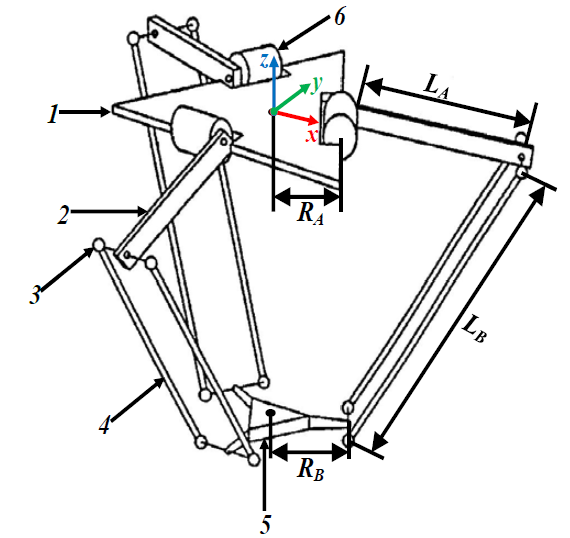
\includegraphics[width=0.5\linewidth]{Main/Chapter4/Images4/Metodo_B_Modelacion_Cinematica_Posicion_1.png}
                  \caption{Fotografía de un paraguas}
                  \label{f:Cap4_Metodo_B_Modelacion_Cinematica_Posicion_1}
            \end{figure}        
        
        
        En la tabla \ref{tab:cap4_tabla_11} muestra la relación entre la numeración en la figura anterior y su descripción:
        
        
        \begin{table}[h]
            \centering
            \begin{tabular}{c c}
            \hline
                \textbf{Numero}& \textbf{Descripción} \\ 
            \hline             \hline
             1 & Base Fija \\
            \hline
             2 & Brazo \\
            \hline
             3 & Junta esférica \\
            \hline
             4 & Antebrazo\\
            \hline
             5 & Efector final \\
             \hline
             6 & Actuador \\
             \hline
            \end{tabular}
           \caption{Referencias del dibujo}
           \label{tab:cap4_tabla_11}
        \end{table}
        
        
        \newpage

        Antes de empezar los cálculos de cinemática, es mejor explicar algunos términos que se utilizará ampliamente en la formulación cinemática.
        
        
         \begin{figure}[htb]
             \centering
              \subfloat[Gatito]{
             \label{f:Cap4_Metodo_B_Modelacion_Cinematica_Posicion_2a}
                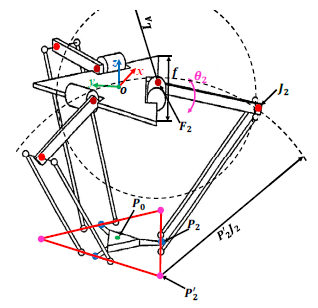
\includegraphics[width=0.5\textwidth]{Main/Chapter4/Images4/Metodo_B_Modelacion_Cinematica_Posicion_2a.png}}
              \subfloat[Tigre]{
             \label{f:Cap4_Metodo_B_Modelacion_Cinematica_Posicion_2b}
                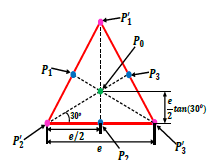
\includegraphics[width=0.4\textwidth]{Main/Chapter4/Images4/Metodo_B_Modelacion_Cinematica_Posicion_2b.png}}
             \caption{Múltiples imágenes}
             \label{f:Cap4_Metodo_B_Modelacion_Cinematica_Posicion_2}
        \end{figure}
        
        
        Los parámetros necesarios para resolver la cinemática del robot delta se presentan en la ilustración \ref{f:Cap4_Metodo_B_Modelacion_Cinematica_Posicion_2} y la  tabla \ref{tab:cap4_tabla_12}:
        
        \begingroup
            \renewcommand{\arraystretch}{1.5}
            \begin{table}[H]
            \centering
            \begin{tabular}{c m{12cm}}
               \hline
               \textbf{Parametro}  & \multicolumn{1}{c}{\textbf{Descripción}}  \\
               \hline           \hline            
             $L_A$ & Largo del brazo \\
            \hline
             $L_B$ & Largo del antebrazo \\
            \hline
             $R_A$ & Distancia entre el centro de la base fija y la junta revoluta o actuador \\
            \hline
             $R_B$ & Distancia entre el centro del efector a la junta que lo une con el antebrazo\\
            \hline
             $f$ & longitud de un lado del triángulo equilátero inscribe el círculo formado por los puntos $F'_1$, $F'_2$ y $F'_3$ (base fija)\\
            \hline
             $e$ & longitud de un lado del equilátero triángulo inscribe el círculo formado por los puntos $P'_1$, $P'_2$ y $P'_3$ (efector final)\\
            \hline
             $\theta_i$ & Angulo de los actuadores\\
            \hline
             $J_i$ & Punto de la junta esférica que conecta los brazos con el antebrazo\\
            \hline            
             $F_i$ & Punto de la posición de los actuadores\\
            \hline  
             $P_0$ & posición del final efector en el espacio cartesiano con respecto al sistema de coordenadas con origen $O$ en el centroide de la base fija\\
            \hline            
            \end{tabular}
            \caption{Referencias del dibujo}
           \label{tab:cap4_tabla_12}
        \end{table}
        \endgroup     
        
        
        \newpage

\subsubsection{Cinemática Directa}\label{mb_cd}
        
        En\ la cinemática directa, se calcula la posición del efector final del manipulador robótico a partir de la información dada de los ángulos en los actuadores.


        \begin{equation}
            \theta _{1},~ \theta _{2}, \theta _{3}~~~ \rightarrow ~  {P_{0}} \left( P_{0x},P_{0y},P_{0z} \right)
        \label{eq:cap4_MB_1}
        \end{equation}

        El método de solución de la cinemática directa en esta sección es el mismo que el empleado para la metodología A de este capitulo. Lo único que cambia es la nomenclatura de los parámetros y la orientación del sistema de referencia local.
        
            \begin{figure}[htb]
                 \centering
                 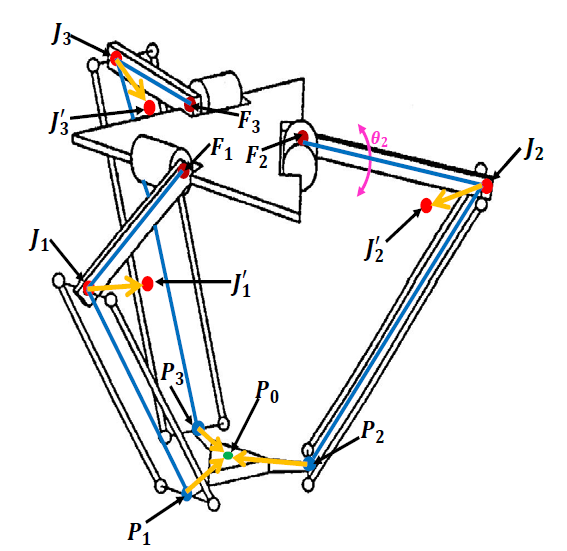
\includegraphics[width=0.7\linewidth]{Main/Chapter4/Images4/Metodo_B_Modelacion_Cinematica_Posicion_3.png}
                  \caption{Fotografía de un paraguas}
                  \label{f:Cap4_Metodo_B_Modelacion_Cinematica_Posicion_3}
            \end{figure}        
        
    Al igual que metodo A, el resultado de las traslaciones de las 3 esferas con centros en las juntas esféricas  \( J_{1},~J_{2},J_{3} \)  producen tres nuevas esferas con radio  \( L_{B} \)  y centro en los puntos  \( J'_{1},~J'_{2},J'_{3} \)   que se cruzan en el punto  \( P_{0} \) . Las coordenadas del vector  \( \overrightarrow{P_{0}}=  \left[ P_{0x},P_{0y},P_{0z} \right] ^{T} \)  se pueden obtener resolviendo las tres ecuaciones que representan las nuevas esferas en el espacio cartesiano simultáneamente. Las ecuaciones son        
        \begin{equation}
            \left( P_{0x}-J'_{ix} \right) ^{2}+ \left( P_{0y}-J'_{iy} \right) ^{2}+ \left( P_{0z}-J'_{iz} \right) ^{2}=L_{B}^{2}~
        \label{eq:cap4_MB_2}
        \end{equation}        
  
    Por lo tanto, se dispone de un sistema de ecuaciones con 3 ecuaciones (\ref{eq:cap4_MB_2}) para $i=1,2,3$ y con 3 incógnitas \( P_{0x},P_{0y},P_{0z} \) .  
    
    \newpage

    Las coordenadas de los puntos  \( J'_{1},~J'_{2},J'_{3} \)  encuentra en los siguientes vectores  (\ref{eq:cap4_MB_3}), (\ref{eq:cap4_MB_4}) y (\ref{eq:cap4_MB_5}) respectivamente:  
  
          \begin{equation}
                \overrightarrow{J'_{1}}= \left [\left( \frac{(f-e)}{2\sqrt{3}}+{L}_{A}cos(\theta_1)\right) cos(30^\circ), \left(\frac{(f-e)}{2\sqrt{3}} + {L}_{A}cos(\theta_1)\right) sin(30^\circ), -L_{A}sin(\theta_1)\right]
        \label{eq:cap4_MB_3}
        \end{equation}    
        
        \begin{equation}
                \overrightarrow{J'_{2}}= \left [  0,-\frac{(f-e)}{2\sqrt{3}}-L_{A}cos(\theta_2),-L_{A}sin(\theta_2)\right]
        \label{eq:cap4_MB_4}
        \end{equation}    
        
        \begin{equation}
                \overrightarrow{J'_{3}}= \left [\left( \frac{(f-e)}{2\sqrt{3}}+{L}_{A}cos(\theta_3)\right) cos(30^\circ), \left(\frac{(f-e)}{2\sqrt{3}} + {L}_{A}cos(\theta_3)\right) sin(30^\circ), -L_{A}sin(\theta_3)\right]
        \label{eq:cap4_MB_5}
        \end{equation}    
  
      El método algebraico para resolver el sistema de ecuaciones (\ref{eq:cap4_MB_2}), en otras palabras, la intersección de las 3 esferas trasladadas, es el mismo que en el metodo A, especificamente desde la ecuación (\ref{eq:cap4_eq_2}).
  
 \newpage
        
        

\subsubsection{Cinemática Inversa}\label{mb_ci}

      En la cinemática inversa, se calculan los ángulos de las articulaciones, en este caso, los actuadores gracias a la posición dada de efector final en el espacio cartesiano. 
      
        \begin{equation}
              P_{0} \left( P_{0x},P_{0y},P_{0z} \right) ~~ \rightarrow    \theta _{1},~ \theta _{2}, \theta _{3} 
        \label{eq:cap4_MB_6}
        \end{equation}\par      
      
     En esta sección, el método de solución de la cinemática inversa es el mismo que el empleado para la metodología A de este capitulo. Lo único que cambia es la nomenclatura de los parámetros y la orientación del sistema de referencia local.
  
           \begin{figure}[htb]
             \centering
              \subfloat[Gatito]{
             \label{f:Cap4_Metodo_B_Modelacion_Cinematica_Posicion_4a}
                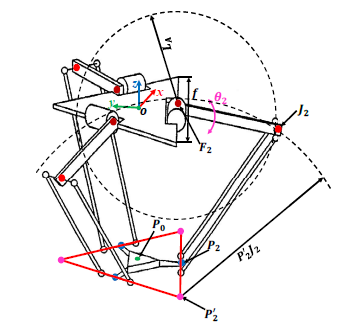
\includegraphics[width=0.5\textwidth]{Main/Chapter4/Images4/Metodo_B_Modelacion_Cinematica_Posicion_4a.png}}
              \subfloat[Tigre]{
             \label{f:Cap4_Metodo_B_Modelacion_Cinematica_Posicion_4b}
                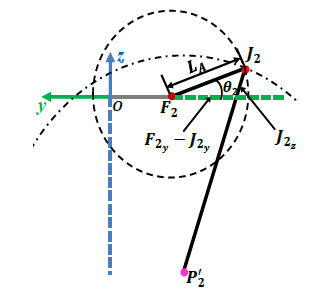
\includegraphics[width=0.4\textwidth]{Main/Chapter4/Images4/Metodo_B_Modelacion_Cinematica_Posicion_4b.png}}
             \caption{Múltiples imágenes}
             \label{f:Cap4_Metodo_B_Modelacion_Cinematica_Posicion_4}
        \end{figure}
  
      Primero se empieza por calcular en ángulo del actuador 2. Se trabaja sobre el marco de referencia $YZ$ ya que el brazo  \overline{\( F_{2}J_{2}  \)} solo puede moverse en ese plano como se muestra en la ilustracion \ref{f:Cap4_Metodo_B_Modelacion_Cinematica_Posicion_4a}. Sobre el mismo plano $ YZ $ se proyecta el antebrazo para obtener una segunda restricción geométrica en la junta  \( J_{2} \) . Por lo explicado anteriormente, la posición de la junta esférica  \( J_{2} \)  está restringida por 2 circunferencias. Se dibuja el primer círculo con centro  \( F_{2} \)  y radio  \( L_{A} \) . El segundo círculo se dibuja con el centro en el punto  \( P'_{2} \) ( proyección de $P_{2}$ sobre plano $YZ$)  y radio  \( \sqrt[]{L_{B}^{2}-P_{0x}^{2}} \) .
      
     \newpage

      La ecuación \ref{eq:cap4_MB_7} y\ref{eq:cap4_MB_8} representan los círculos con radio  \( L_{A} \)  y  \( \sqrt[]{L_{B}^{2}-P_{0x}^{2}} \)  respectivamente, como se muestra en la figura \ref{f:Cap4_Metodo_B_Modelacion_Cinematica_Posicion_4b}.
  
  
        \begin{equation}
              (J_{2y}-F_{2y})^2 + (J_{2z}-F_{2z})^2=  L_{A}^{2}  \Rightarrow  \left (J_{2y} + \frac{f}{2\sqrt{3}}\right)^2 + J_{2z}^{2}= L_{A}^{2}
        \label{eq:cap4_MB_7}
        \end{equation}
        
        
        \begin{equation} 
              (J_{2y}-{P'}_{2y})^2 + (J_{2z}-{P'}_{2z})^2= L_{B}^{2} -P_{0z}^2  \Rightarrow   \left (J_{2y} - P_{0y}+ \frac{e}{2\sqrt{3}}\right)^2 + ({J}_{2z}-{P}_{0z}) = L_{B}^{2} -P_{0z}^2
        \label{eq:cap4_MB_8}
        \end{equation}  
    
    
        El valor de  \( J_{2y} \)  y  \( J_{2z} \)  se puede calcular resolviendo simultáneamente la ecuación \ref{eq:cap4_MB_7} y \ref{eq:cap4_MB_8} al igual que en el metodo A. Todas las demás variables en este sistema de ecuaciones se asumen como conocidas o se miden a partir de la estructura geométrica del robot paralelo delta. Una vez que se conocen estos valores, se puede usar trigonometría simple para calcular el  \(  \theta _{2} \)  como se indica en la siguiente ecuacion \ref{}:
        
        \begin{equation} 
            \theta_2=arctan \left(\frac{J_{2z}}{{F}_{2y}-{J}_{2y}}\right)
        \label{eq:cap4_MB_9}
        \end{equation}  
   
   
        La estructura simétrica del robot paralelo delta da la ventaja de calcular los ángulos  \(  \theta _{1} \)  y  \(  \theta _{3} \)  faltantes aplicando el mismo procedimiento para  \(  \theta _{2} \) . Para ello, se rotar el marco de referencia local en un ángulo de 120º en sentido antihorario y horario, respectivamente.   
           
     
        \newpage

\subsection{Modelación cinemática de la velocidad}\label{mb_cvel}
    
        Con el objetivo de modelar la cinemática de velocidad del robot delta, en esta sección se implementa las ideas expuestas en la fuente \cite{Path_Planning_and_Trajectory_Optimization},  con los mismos parámetros, jerga y nomenclatura de la seccion  \ref{MB_MP}
        La base de la modelacion cinematica de velocidad es determinar la matriz jacobiana  \( J \) . Esta juega un papel importante en el modelo dinámico del manipulador robótico como se aprecia en secciones posteriores.\par
        
        La matriz jacobiana para el robot paralelo delta fue calculada por primera vez por Codourey \cite{Codourey:31400}. En este método, las derivadas parciales se calcularon numéricamente. La matriz jacobiana para robots paralelos también se puede calcular vinculando la variable de espacio cartesiano con las variables de espacio de articulación mediante un conjunto de ecuaciones restringidas. Guglielmetti \cite{Guglielmetti:31706} fue la primera persona que aplicó este enfoque para calcular la matriz jacobiana para el robot paralelo Delta. Codourey \cite{DynamicCodourey} aborda una versión simplificada de la formulación de Guglielmetti. En esta tesis, se adopta el método de Codourey para calcular la matriz jacobiana.

        \subsubsection{Jacobiano}

        La matriz jacobiana $J$ describe la relación entre las velocidades espaciales cartesianas y las velocidades articulares como se indica en la ecuación (\ref{eq:cap4_MB_10}).

        \begin{equation} 
            \overrightarrow{\dot{P_{0}}}=J\overrightarrow{\dot{ \theta }}~ 
            \label{eq:cap4_MB_10}
        \end{equation}  
   
        Para encontrar una expresión de la matriz jacobiana, se utilizar la longitud del antebrazo de un robot paralelo delta como una ecuación de restricción.

        \begin{equation} 
            \overrightarrow{s_{i}}^T \cdot \overrightarrow{s_{i}} - L_{B}^{2} = 0
            \label{eq:cap4_MB_11}
        \end{equation} 

            \begin{figure}[htb]
                 \centering
                 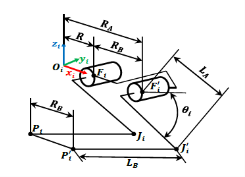
\includegraphics[width=0.4\linewidth]{Main/Chapter4/Images4/Metodo_B_Modelacion_Cinematica_Posicion_5.png}
                  \caption{Fotografía de un paraguas}
                  \label{f:Cap4_Metodo_B_Modelacion_Cinematica_Posicion_5}
            \end{figure}  

        \newpage
        Donde: 
        
    \begin{align}
        \overrightarrow{s_{i}} & = \overrightarrow{P_{0}}- \left(\overrightarrow{F_{i}}+\overrightarrow{\xi_{F_{i}J_{i}}} \right)\\&= 
            \begin{bmatrix}
                P_{0x} \\
                P_{0y} \\
                P_{0z}
            \end{bmatrix} -  R_{i}^{R}
            \left( 
            \begin{bmatrix}
                R \\
                0\\
                0
            \end{bmatrix} + 
            \begin{bmatrix}
                L_{A} cos(\theta_i) \\
                0\\
                -L_{A} sin(\theta_i) 
            \end{bmatrix}
            \right)
        \label{eq:cap4_MB_12}
    \end{align}
    
    En (\ref{eq:cap4_MB_12}), $[P_{0x},P_{0y},P_{0z}]$ es la posición del efector final $\overrightarrow{P_{0}}$ , y el superíndice $R$ es el marco de referencia local $O-xyz$ como se muestra en la ilustracion \ref{f:Cap4_Metodo_B_Modelacion_Cinematica_Posicion_5}. $R$ es la diferencia entre ${R}_{A}$ y ${R}_{B}$.
    Debido a la simetría en la estructura del robot paralelo delta, cada brazo se puede tratar por separado. Cada brazo está separado por un ángulo de 120° grados y la posición del sistema de referencia correspondiente para cada brazo $O_i - x_i y_i z_i$  es el mismo que el superindice $R$ pero girado en un ángulo para cada brazo $i={1,2 ,3}$, respectivamente. 
    La matriz de transformación  o  la  matriz de rotación se indica en (\ref{eq:cap4_MB_13}).
    
       \begin{equation}
         R_{i}^{R} =
        \begin{bmatrix}
                cos(\varphi_i)&-sin(\varphi_i)&0 \\
                sin(\varphi_i)&cos(\varphi_i)&0 \\
                0&0&1
            \end{bmatrix}
        \label{eq:cap4_MB_13}
    \end{equation}  
    
    
    Derivando la ecuación (\ref{eq:cap4_MB_11})y realizando álgebra básica se llega a la siguiente expresión del jacobiano $J$: 
    
    \begin{equation}
        J = -J_{1}J_{2}=-
        {\begin{bmatrix}
                \overrightarrow{s_{1}}^T \\
                \overrightarrow{s_{2}}^T \\
                \overrightarrow{s_{3}}^T
            \end{bmatrix}}^{-1}
        {\begin{bmatrix}
                \overrightarrow{s_{1}}^{T} \cdot \overrightarrow{b_{1}} &0&0\\
                0 &\overrightarrow{s_{2}}^{T}\cdot \overrightarrow{b_{2}}&0\\
                0 &0&\overrightarrow{s_{3}}^{T}\cdot \overrightarrow{b_{3}}
            \end{bmatrix}}
        \label{eq:cap4_MB_14}
    \end{equation}  
    
    Donde:
    \begin{equation}
        \overrightarrow{b_{i}} = R_{i}^{R}             
        \begin{bmatrix}
                L_{A} sin(\theta_i) \\
                0\\
                L_{A} cos(\theta_i) 
            \end{bmatrix}
        \label{eq:cap4_MB_15}
    \end{equation}  
    
    En el caso de los robots en serie, la matriz jacobiana es solo una función de $\overrightarrow{\theta}$   , pero para los robots paralelos, la matriz jacobiana depende de la información del espacio articular $\overrightarrow{\theta}$   así como de la posición del efector final $\overrightarrow{P_0}$   .
        \newpage

    \subsection{Modelación Cinematica de Aceleracion}
        
        En esta sección se presentan las ecuaciones para determinar la aceleración angular de los actuadores del robot delta. La aceleración se determina derivando 2 veces matricialmente la ecuación (\ref{eq:cap4_MB_11}) de la sección \ref{mb_cvel} de modelación cinemática de velocidad para el método B.
        
        La aceleración angular de los motores del robot delta se calcula con la siguiente formula:
        
        
        \begin{equation}
                    \overrightarrow{\ddot{ \theta }}=J^{-1} \left[ \overrightarrow{\ddot{P_{0}}}+ \left[ \begin{matrix}
                \overrightarrow{s_{1}}^{T}\\
                \overrightarrow{s_{2}}^{T}\\
                \overrightarrow{s_{3}}^{T}\\
                \end{matrix}
                 \right] ^{-1} \ast \left(  \left[ \begin{matrix}
                \overrightarrow{\dot{s}_{1}}^{T}\\
                \overrightarrow{\dot{s}_{2}}^{T}\\
                \overrightarrow{\dot{s}_{3}}^{T}\\
                \end{matrix}
                 \right]  J+K \right) \ast\overrightarrow{\dot{ \theta }} \right]
            \label{eq:cap4_MB_16}
        \end{equation} 

        Donde: 

        \begin{equation}
                 K= \left[ \begin{matrix}
                \overrightarrow{\dot{s}_{1}}^{T}\overrightarrow{b_{1}}+\overrightarrow{s_{1}}^{T}\overrightarrow{\dot{b}_{1}}  &  0  &  0\\
                0  &  \overrightarrow{\dot{s}_{2}}^{T}\overrightarrow{b_{2}}+\overrightarrow{s_{2}}^{T}\overrightarrow{\dot{b}_{2}}  &  0\\
                0  &  0  &  \overrightarrow{\dot{s}_{3}}^{T}\overrightarrow{b_{3}}+\overrightarrow{s_{3}}^{T}\overrightarrow{\dot{b}_{3}}\\
                \end{matrix}
                 \right]  
            \label{eq:cap4_MB_17}
        \end{equation} 
        
        \begin{equation}
                  \overrightarrow{\dot{b}_{i}}= \left[ \begin{matrix}
                L_{A} cos⁡ \left(  \theta _{i} \right) \\
                0\\
                - L_{A}\sin ⁡ \left(  \theta _{i} \right) \\
                \end{matrix}
                 \right] \overrightarrow{\dot{ \theta _{i}}}  
            \label{eq:cap4_MB_18}
        \end{equation} 
        
        \begin{equation}
                  \overrightarrow{\dot{s}_{i}}= \left[ \begin{matrix}
                \dot{P}_{0x}\\
                \dot{P}_{0y}\\
                \dot{P}_{0z}\\
                \end{matrix}
                 \right] +R_{i}^{R}\ast \left[ \begin{matrix}
                L_{A}\sin  \left(  \theta _{i} \right) \\
                0\\
                L_{A}\cos  \left(  \theta _{i} \right) \\
                \end{matrix}
                 \right] \dot{ \theta _{i}}=\overrightarrow{\dot{P_{0}}}+\overrightarrow{b_{i}}~\dot{ \theta _{i}} 
            \label{eq:cap4_MB_19}
        \end{equation} 

        


        








    \newpage

    \subsection{Modelación Dinámica}
    
    \newpage


\section{Espacio de trabajo}

En esta sección se da a conocer la definición de espacio de trabajo por algunos científicos que se han especializado en esta problemática para robots, se presentan de manera general los 2 métodos más utilizados para determinar el espacio y se muestran las restricciones de un robot delta relacionadas con este tema.

    \subsection{Definición}
    En los últimos años, los robots que incluyen una estructura paralela atrajeron la atención de los investigadores del mundo académico. Entre los robots con estructura paralela más famosos se encuentran los provistos de la estructura paralela delta de 3 grados de libertad.  Al comparar los robots que incluyen manipuladores de estructuras en serie con los que incluyen manipuladores de estructuras paralelas, se puede notar que: la estructura paralela tiene una lista de ventajas, como alta rigidez, disponibilidad para transportar objetos más pesados, posicionamiento más preciso, etc. Estas ventajas también vienen dadas por el hecho de que las fuerzas inerciales y de gravedad del objeto manipulado es absorbida por cada enlace cinemático aparte \cite{Laribi08}\cite{DASH2005776}. Las desventajas son: espacio de trabajo más estrecho y un control más difícil \cite{DASH2005776}.  
    
    El espacio de trabajo de un robot se define como la región en el espacio cartesiano tridimensional que puede ser alcanzada por un punto de su efector final \cite{LARIBI2007859}, es decir, en el caso de un robot Delta, es la región en el espacio tridimensional que puede alcanzar el punto central de su plataforma móvil. 
    
    \begin{figure}[htb]
        \centering
        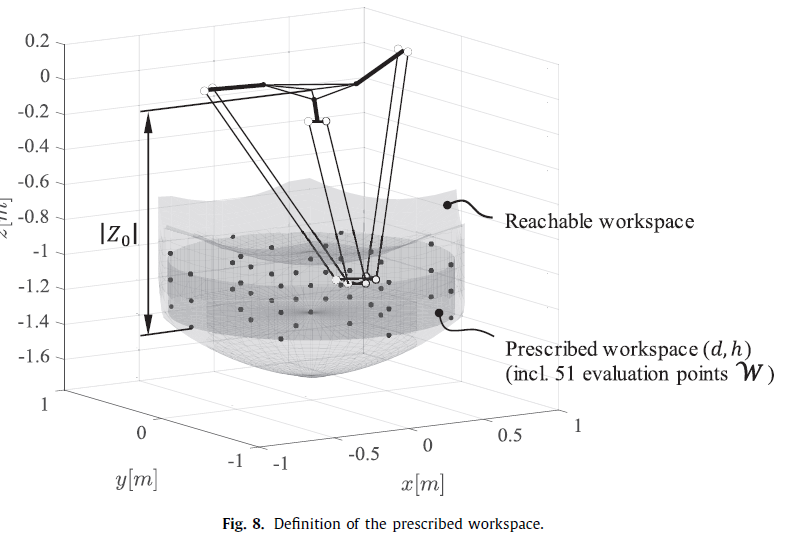
\includegraphics[width=0.7\linewidth]{Main/Chapter4/Images4/cap4_ws_1.png}
        \caption{Fotografía de un paraguas}
        \label{f:Cap4_ws_1}
    \end{figure}  
    
    \newpage
    
    \subsection{Métodos}
    
    El espacio de trabajo de los robots ha sido estudiado intensamente a lo largo de los años por varios investigadores. Los espacios de trabajo más comunes, según Merlet, son: el espacio de trabajo de traducción, el espacio de trabajo de orientación, el espacio de trabajo accesible, el espacio de trabajo de orientación inclusiva, el espacio de trabajo de orientación total, el espacio de trabajo de destreza, el espacio de trabajo total con orientación reducida \cite{Laribi08} y \cite{AFFI2004311}.
    
    Se han utilizado básicamente las siguientes categorías de métodos para determinar el espacio de trabajo: métodos geométricos y métodos de digitalización, siendo este último el más usado.
    El método geométrico \cite{delta_Urrea} se basa en obtener un objeto geométrico que describa todas las posibles posiciones del efector final y que satisfagan las restricciones del robot. Se obtiene un objeto geométrico para cada cadena cinemática del robot y el espacio de trabajo es la intersección de los objetos geométricos obtenidos.
    
    El método de discretización \cite{delta_Urrea}, que se basa en métodos numéricos, consiste en discretizar el espacio en tres dimensiones, resolviendo la cinemática inversa para cada punto y verificando las restricciones que limitan dicho espacio de trabajo (Ottaviano and Ceccarelli, 2000). La exactitud del volumen de trabajo del robot Delta, depende de la probabilidad de que los puntos seleccionados aleatoriamente puedan ser alcanzados por el robot. 
    
    En esta tesis se basa en el método de discretización, sin embargo, será modificado para que el algoritmo calcule la cantidad exacta de los puntos en el espacio que es capaz de alcanzar la plataforma móvil del robot \cite{delta_Urrea}. El algoritmo se basa en la solución de la cinemática directa para todas las posibles combinaciones de los actuadores, obteniendo en cada caso un punto en el espacio. El punto pertenece al espacio de trabajo del robot sí y solo sí cumple con todas las restricciones impuestas.
    
    \newpage

    
    \subsection{Tipos de restricciones}\label{restriccionesWS}
    El movimiento de los robots manipuladores dentro del espacio de trabajo puede estar restringido por varios factores, tales como: los límites constructivos de los acoplamientos cinemáticos pasivos, los límites dados por los dispositivos de accionamiento de los acoplamientos cinemáticos activos, las cohesiones dadas por los elementos constructivos del robot, así como por puntos o áreas de singularidad que pueden dividir el espacio de trabajo en varios componentes \cite{Laribi08}. 
    
    Las restricciones que se toman en cuenta en este documento para determinar el espacio de trabajo del robot delta son principalmente: 
   
    \begin{itemize}
    	\item Limites impuesto de los ángulos de los actuadores [  \(  \theta _{1i,min} \)  -   \(  \theta _{1i,max} \)  ] para cada actuador  \( i= \{ 1,2,3 \}  \)  .\par
    
    	\item Resolución basada en tamaño del paso de los actuadores, es decir, la discretización del rango impuesto por los límites del punto anterior  \(  \Delta  \theta _{1i} \)  para cada actuador  \( i= \{ 1,2,3 \}  \) .\par
    
    	\item Restricciones de ángulos internos en base a restricción de las juntas o rotulas  \(  \theta _{2i} \)  y  \(  \theta _{3i} \) .\par
    
    	\item Singularidades que se determinan mediante el determinante del jacobiano  \( J=J_{x}^{-1}J_{ \theta } \)   cuando este es cercano a 0. Estas singularidades son las mismas explicadas en la sección \ref{CAP4_SINGULARIDAD}.
    	
    	\item Restricciones limites impuestas por el fabricante. Generalmente son volúmenes geométricos como cilindros o cubos.	
    	
    \end{itemize}
    
    
    En la ilustracion \ref{f:Cap4_ws_2} se visualizan de mejor manera las restricciones a considerar:
    
    
    \begin{figure}[htb]
        \centering
        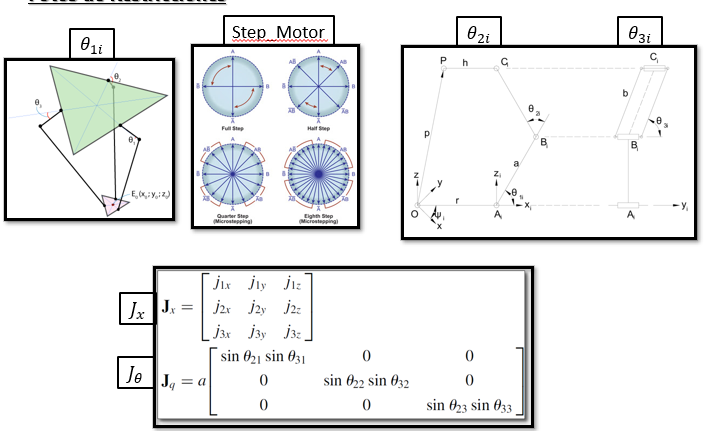
\includegraphics[width=0.6\linewidth]{Main/Chapter4/Images4/cap4_ws_2.png}
        \caption{Fotografía de un paraguas}
        \label{f:Cap4_ws_2}
    \end{figure}   

    \newpage

\section{Trayectorias}\label{cap4_tray}

    El objetivo principal de esta sección es explicar de manera general la implementación de las trayectorias en robots y dar a conocer detalladamente la trayectoria que se utiliza en este trabajo de grado.
    
    En primer lugar, se define que es una trayectoria, se exponen sus objetivos y se propone un diagrama de flujo con relación a los pasos que se realizan para obtenerlas.
    
    En segundo lugar, se presentan 5 clasificaciones de trayectorias más comunes por los científicos y expertos en robótica para todo tipo de robots.
    
    Finalmente, se describe la trayectoria como la combinación de 2 partes: una descripción puramente geométrica de la secuencia de configuraciones logradas por el robot y una escala de tiempo que especifica los tiempos en que se alcanzan esas configuraciones. A partir del punto de vista anterior, se consideran el caso de las trayectorias punto a punto tanto en el espacio de articulaciones como en el espacio de cartesiano.
    
    \subsection{Definición de trayectorias}
        Un camino geométrico $p$ es un conjunto de puntos en el espacio articular o cartesiano que un manipulador de un robot debe seguir, en otras palabras, es una descripción puramente geométrica. La ecuación (\ref{eq:cap4_tray_1}) representa un camino geométrico en el espacio cartesiano: 

        \begin{equation}
            p(s) = [x(s), y(s), z(s)]^T
        \label{eq:cap4_tray_1}
    \end{equation}  
    
    Una trayectoria es un camino geométrico $p(s)$  más consideraciones temporales $s(t)$ . Estas consideraciones temporales pueden estar restringidas por velocidades o aceleraciones impuestas a lo largo del camino. Usualmente se escoge un camino y luego se escoge la ley temporal para la trayectoria.
    
    \begin{equation}
            p(s(t)) = [x(s(t)), y(s(t)), z(s(t))]^T
        \label{eq:cap4_tray_2}
    \end{equation}  
    
    
    \begin{figure}[htb]
        \centering
        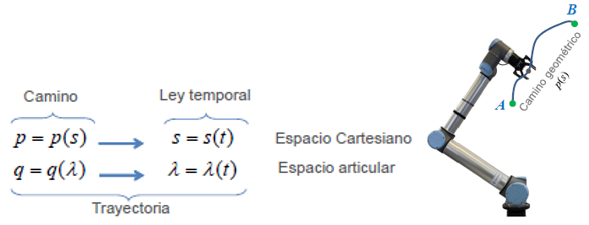
\includegraphics[width=0.7\linewidth]{Main/Chapter4/Images4/cap4_tray_1.png}
        \caption{Fotografía de un paraguas}
        \label{f:Cap4_tray_1}
    \end{figure}    
    
    \newpage
    
    \subsection{Nomenclatura de trayectorias}
        Un camino geométrico $\theta(s)$ esta en función de un parámetro de camino escalar $s$, que asume que es $0$ al comienzo del camino y $1$ al final, en un punto en el espacio de configuración del robot $\Theta$.
        
    \begin{equation}
        \theta: s \rightarrow   \Theta 
        \label{eq:cap4_tray_3}
    \end{equation}  
    
        \begin{equation}
        \theta: [0;1] \rightarrow   \Theta
        \label{eq:cap4_tray_4}
    \end{equation}
    
    A medida que $s$ aumenta de $0$ a $1$, el robot se mueve a lo largo de la trayectoria. A veces, $s$ se toma como tiempo y se permite que varíe desde el tiempo $s=0$ hasta el tiempo total de movimiento $s=T$, pero a menudo es útil separar el papel del parámetro de trayectoria geométrica $s$  del parámetro de tiempo $t$. Una escala de tiempo $s(t)$ se le asigna un valor $s$ a cada tiempo $t$ $ \in [0; T]$:

    \begin{equation}
        s: t \rightarrow   [0;1] 
        \label{eq:cap4_tray_5}
    \end{equation}  
    
        \begin{equation}
        s: [0; T] \rightarrow   [0;1] 
        \label{eq:cap4_tray_6}
    \end{equation}


    Juntos, un camino geométrico $\theta(s)$ y una escala de tiempo $s(t)$  definen una trayectoria $\theta(s(t))$  o $\theta(t)$   para abreviar. Usando la regla de la cadena, la velocidad y la aceleración a lo largo de la trayectoria se pueden escribir como:


    \begin{equation}
        \dot{\theta} = \frac{d\theta}{ds} \dot{s}
        \label{eq:cap4_tray_7}
    \end{equation}  
    
        \begin{equation}
        \ddot{\theta} = \frac{d\theta}{ds} \ddot{s} + \frac{d^2\theta}{ds^2} \dot{s}^2
        \label{eq:cap4_tray_8}
    \end{equation}


    Para asegurar que la aceleración del robot (y por lo tanto la dinámica) esté bien definida, $\theta(s)$ y $s(t)$ deben ser dos veces diferenciales.

    \newpage
    
    \subsection{Objetivo y procedimiento de generación de trayectorias}
    
    El control cinemático en robótica es una herramienta que permite establecer cuáles son las trayectorias que debe seguir cada articulación del robot a lo largo del tiempo para conseguir los objetivos fijados por el usuario, tales como:
    
    \begin{itemize}
        \item 	Punto de destino
         \item  Tipo de trayectoria del extremo
         \item  Tiempo total invertido

    \end{itemize}
    
    
    Para ello es necesario tomar en cuenta las restricciones físicas de los accionamientos y criterios de calidad tales como sensibilidad, precisión, repetitividad, etc.
    
    Un procedimiento típico para la generación de trayectorias en robots es el que se aprecia en la ilustracion \ref{f:Cap4_tray_3}:
    
    \begin{figure}[htb]
        \centering
        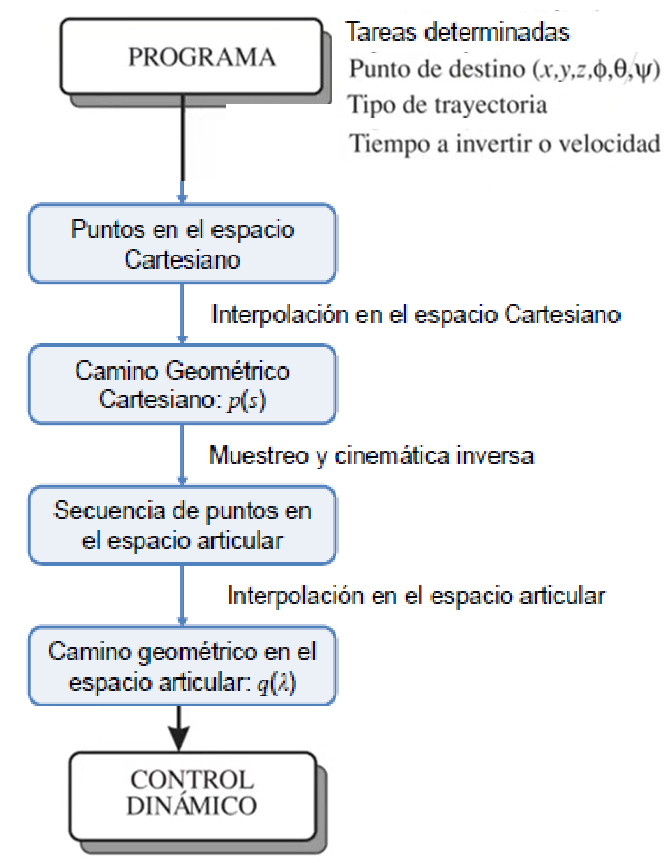
\includegraphics[width=0.65\linewidth]{Main/Chapter4/Images4/cap4_tray_3.png}
        \caption{Fotografía de un paraguas}
        \label{f:Cap4_tray_3}
    \end{figure}  
    
    

        \newpage

    \subsection{Clasificación de trayectorias}
        En esta sección se presentan 5 clasificaciones mas utilizadas para agrupar las trayectorias todo tipo de robots:
        
        \subsubsection{Según el espacio }
            Según la importancia que se le asigna al camino de la trayectoria de un brazo robótico o un efector final de un punto inicial a un punto final en una tarea específica, se pueden dividir en 2 grupos: trayectorias cartesianas y trayectorias articulares. Las trayectorias cartesianas se utilizan cuando es necesario que el robot siga una determinada trayectoria geométrica. Acerca de estas trayectorias, es importante recalcar que sirven para evitar obstáculos, la visualización del camino generado es más fácil y requiere de cinemática inversa. Por el contrario, las trayectorias articulares se ocupan cuando se requiere ir de un punto a otro sin importar la trayectoria. 
            
           \begin{figure}[htb]
             \centering
             \label{f:cap4_tray_4a}
                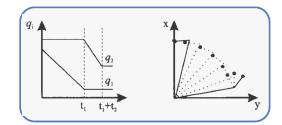
\includegraphics[width=0.6\textwidth]{Main/Chapter4/Images4/cap4_tray_4a.png}
             \caption{Múltiples imágenes A}
        \end{figure}            


           \begin{figure}[htb]
             \centering
             \label{f:cap4_tray_4b}
                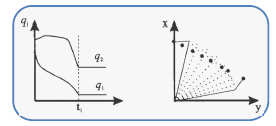
\includegraphics[width=0.6\textwidth]{Main/Chapter4/Images4/cap4_tray_4b.png}
             \caption{Múltiples imágenes B}
        \end{figure}         
            
            
         \newpage   
        
        \subsubsection{Según la geometría del camino }
            El punto de vista principal de esta clasificación es en la forma de la función que representa la trayectoria, ya sea cartesiana o articular. Existen muchos tipos, algunos de estos son:
            \begin{itemize}
                \item         Trayectorias rectilíneas
                \item        Trayectorias polinomiales
                \item        Trayectorias exponenciales
                \item        Trayectorias cicloides
            \end{itemize}
                
        \begin{figure}[htb]
            \centering
            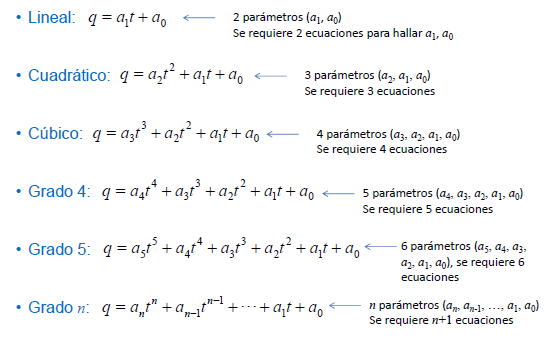
\includegraphics[width=1\linewidth]{Main/Chapter4/Images4/cap4_tray_5.png}
            \caption{Fotografía de un paraguas}
            \label{f:Cap4_tray_5}
        \end{figure}              
            
        \newpage   

        
        \subsubsection{Según la ley temporal }
            Esta clasificación se basa en las especificaciones de puntos en el camino (velocidades, posición donde detenerse), restricciones impuestas por los actuadores o tareas especificadas (máximo torque, máxima velocidad) o en considerar criterios de optimización (mínimo tiempo, mínima energía o una combinación de ambos).  Ejemplos de aquellas son:
            \begin{itemize}
                \item   Trayectorias tipo bang-bang (on/off) en aceleración
                \item   Trayectorias trapezoidales en velocidad
                \item   Trayectorias polinomiales
            \end{itemize}
            
           \begin{figure}[htb]
             \centering
              \subfloat[Gatito]{
             \label{f:cap4_tray_6a}
                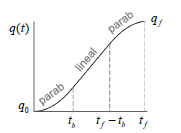
\includegraphics[width=0.5\textwidth]{Main/Chapter4/Images4/cap4_tray_6a.png}}
              \subfloat[Tigre]{
             \label{f:cap4_tray_6b}
                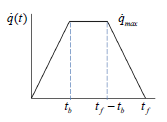
\includegraphics[width=0.5\textwidth]{Main/Chapter4/Images4/cap4_tray_6b.png}}
             \caption{Múltiples imágenes}
             \label{f:cap4_tray_6}
        \end{figure}            
            
            
            
        
        \subsubsection{Según la coordinación }
            Esta categoría toma toda la atención a la sincronía que tienen las articulaciones en un desplazamiento de un robot de un punto a otro. Se puede dividir en dos grupos: trayectorias coordinadas e independientes. Las trayectorias coordinadas se refieren a que todas las articulaciones inician y terminan el movimiento al mismo tiempo y en simultáneo, mientras que las trayectorias independientes el movimiento de cada articulación es independiente.
        
                 \newpage   

        
        
        \subsubsection{Según el tipo de tarea }
            Dependiendo de la tarea que se quiera realizar, se pueden subdividir en 3 tipos las trayectorias según los puntos por los que debe recorrer el efector final o el ultimo brazo del robot en el espacio cartesiano o articular:

            \begin{itemize}
                \item 	 Trayectorias punto a punto: ir de un punto a otro sin importar la trayectoria 
                \item 	 Trayectorias de puntos vías: ir de un punto a otro, pero pasando por puntos intermedios
                \item 	 Trayectorias continuas (continuidad de velocidad, aceleración): ir de un punto a otro por una trayectoria especifica teóricamente de puntos infinitos
            \end{itemize}
        

    \subsection{Trayectorias punto a punto}
        El tipo de movimiento más simple es desde el reposo en una configuración hasta el reposo en otra. A esto lo llamamos movimiento de punto a punto. El tipo de trayectoria más simple para el movimiento de punto a punto es una línea recta. Las rutas en línea recta y sus escalas de tiempo se analizan a continuación. Las ideas en esta seccion son extraidas del libro creado por los academicos de la Universidad de Northwestern  \cite{moder_robot}.
    
        \subsubsection{Trayectorias en Linea Recta}
            Una línea recta comienza con una configuración inicial $\theta_{inicio}$ hasta una configuración final $\theta_{fin}$ que pueden ser definidas en espacio de articulaciones o en espacio cartesiano. La línea recta se puede escribir: 
        
            \begin{equation}
                \theta(s)= \theta_{inicio} + s(\theta_{fin}-\theta_{inicio}) ; s \in [0,1]
                \label{eq:cap4_tray_9}
             \end{equation}
            
            Sus derivadas son:
            \begin{equation}
                \frac{d\theta}{ds}=\theta_{fin}-\theta_{inicio}
                \label{eq:cap4_tray_10}
             \end{equation}      
            \begin{equation}
                \frac{d^2\theta}{ds^2}=0
                \label{eq:cap4_tray_11}
             \end{equation}  
            
            Las líneas rectas en el espacio articular generalmente no producen un movimiento en línea recta del efector final en el espacio cartesiano. Si se desean movimientos en línea recta en el espacio cartesiano, $X_{inicio}$ y $X_{fin}$ pueden especificar las configuraciones de inicio y finalización. Si $X_{inicio}$ y $X_{fin}$ están representados por un conjunto mínimo de coordenadas, entonces una línea recta se define como:
            
            \begin{equation}
                X(s)= X_{inicio} + s(X_{fin}-X_{inicio}) ; s \in [0,1]
                \label{eq:cap4_tray_12}
             \end{equation}    
                
            \begin{figure}[htb]
                \centering
                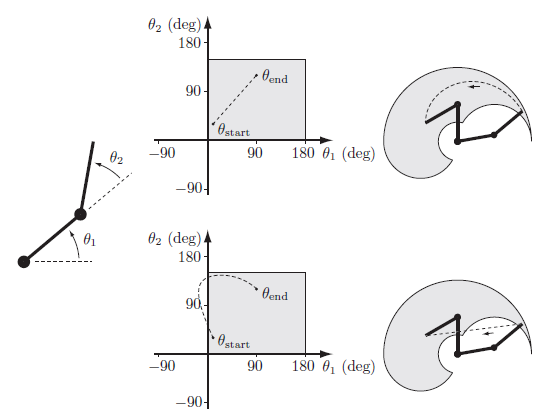
\includegraphics[width=1\linewidth]{Main/Chapter4/Images4/cap4_tray_7.png}
                \caption{Fotografía de un paraguas}
                \label{f:Cap4_tray_7}
            \end{figure}  
            
        En comparación con el caso en el que se utilizan coordenadas articuladas, se deben abordar las siguientes cuestiones:
        \begin{itemize}
                \item Si el camino pasa cerca de una singularidad cinemática, las velocidades de las articulaciones pueden volverse excesivamente grandes para la mayoría de las escalas de tiempo del camino.
                \item Dado que el espacio de trabajo en el que se desenvuelve el efector final de un robot puede no ser convexo en coordenadas X, algunos puntos en una línea recta entre dos puntos finales alcanzables pueden no ser accesibles. 
        \end{itemize}

        \newpage

            
            
            
        \subsubsection{Escala temporal de un camino en línea recta}
            Una escala de tiempo $s(t)$ de una trayectoria debe garantizar que el movimiento sea lo suficientemente suave y que se satisfaga cualquier restricción sobre la velocidad y aceleración del robot. Para una trayectoria en línea recta en el espacio articular de la forma de la ecuacion (\ref{eq:cap4_tray_9}), las velocidades y aceleraciones articulares escaladas en el tiempo son respectivamente:
        
        
            \begin{equation}
                \dot{\theta}=\dot{s} (\theta_{fin}-\theta_{inicio})
                \label{eq:cap4_tray_13}
             \end{equation}      
             
            \begin{equation}
                \ddot{\theta}=\ddot{s} (\theta_{fin}-\theta_{inicio})
                \label{eq:cap4_tray_14}
             \end{equation}  
        
    Para un camino en línea recta en el espacio cartesiano parametrizado por un conjunto mínimo de coordenadas $X\in{\Re}^m$, simplemente se reemplaza $\theta$, $\dot{\theta}$,$\ddot{\theta}$ por $X$, $\dot{X}$,$\ddot{X}$ .        
        
        \paragraph{Escala de tiempo polinomial}
        
            Una forma conveniente para la escala de tiempo $s(t)$ es un polinomio cúbico en función del tiempo: 
            
            \begin{equation}
                s(t)= a_{0}+a_{1}t+a_{2}t^{2}+a_{3}t^{3}
                \label{eq:cap4_tray_15}
             \end{equation}     
        
            Un movimiento de punto a punto desde el tiempo $0$ al  $T$ imponer las restricciones iniciales:
        
            \begin{equation}
                s(0)= \dot{s}(0) = 0 
                \label{eq:cap4_tray_16}
             \end{equation} 
             
             y las restricciones terminales:
             
            \begin{equation}
                s(T) = 1 
                \label{eq:cap4_tray_17}
             \end{equation} 
            \begin{equation}
                \dot{s}(T) = 0 
                \label{eq:cap4_tray_18}
             \end{equation}         
             
            Derivando la ecuación (\ref{eq:cap4_tray_15}):
            \begin{equation}
                \dot{s}(t)= a_{1}+2a_{2}t+3a_{3}t^{2}
                \label{eq:cap4_tray_19}
             \end{equation}     
            
        Evaluando la ecuación (\ref{eq:cap4_tray_19}) en  $t = 0$ , $t = T$ y resolviendo las cuatro restricciones (\ref{eq:cap4_tray_16}),(\ref{eq:cap4_tray_17}),(\ref{eq:cap4_tray_18}) :
        
            \begin{equation}
                 a_{0}=0;a_{1}=0;a_{2}=\frac{3}{T^2};a_{3}=-\frac{2}{T^3}
                \label{eq:cap4_tray_20}
             \end{equation}     
        
        Reemplazando los coeficientes $a_i$ en la ecuación (\ref{eq:cap4_tray_15}): 
        
            \begin{equation}
                s(t)=a_{2}t^{2}+a_{3}t^{3} = (\frac{3}{T^2})t^{2}+(-\frac{2}{T^3})t^{3}
                \label{eq:cap4_tray_21}
             \end{equation}  
             

            Sustituyendo la ecuación (\ref{eq:cap4_tray_21}) y sus derivadas en las ecuaciones (\ref{eq:cap4_tray_9}),(\ref{eq:cap4_tray_13}) y  (\ref{eq:cap4_tray_14}) :
            
            \begin{equation}
                \theta(t)= \theta_{inicio} + \left(  \frac{3t^{2}}{T^2}-\frac{2t^{3}}{T^3} \right) (\theta_{fin}-\theta_{inicio})            
                \label{eq:cap4_tray_22}
             \end{equation}   
             
            \begin{equation}
                  \dot{\theta}(t)= \left(  \frac{6t}{T^2}-\frac{6t^{2}}{T^3} \right) (\theta_{fin}-\theta_{inicio})
                \label{eq:cap4_tray_23}
             \end{equation} 
             
            \begin{equation}
                \ddot{\theta}(t)= \left(  \frac{6}{T^2}-\frac{12t}{T^3} \right) (\theta_{fin}-\theta_{inicio})
                \label{eq:cap4_tray_24}
             \end{equation} 
             
             \begin{figure}[htb]
                \centering
                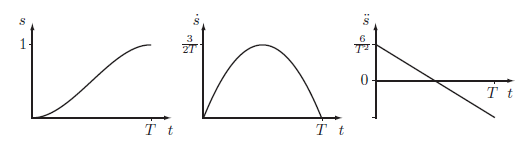
\includegraphics[width=0.8\linewidth]{Main/Chapter4/Images4/cap4_tray_8.png}
                \caption{Fotografía de un paraguas}
                \label{f:Cap4_tray_8}
            \end{figure}  
             
             
        Las velocidades máximas de la articulación se alcanzan en el punto medio del movimiento, $t = T/2$ : 
        
            \begin{equation}
                  {\dot{\theta}}_{max}= \frac{3}{2T} (\theta_{fin}-\theta_{inicio})
                \label{eq:cap4_tray_25}
             \end{equation} 

        Las aceleraciones y desaceleraciones máximas de la articulación se logran en $t = 0$ y $t = T$:
        
            \begin{equation}
                  {\ddot{\theta}}_{max}= \left | { \frac{6}{T^2} (\theta_{fin}-\theta_{inicio})} \right|
                \label{eq:cap4_tray_26}
             \end{equation} 
        
            \begin{equation}
                  {\ddot{\theta}}_{min}= -\left | { \frac{6}{T^2} (\theta_{fin}-\theta_{inicio})} \right|
                \label{eq:cap4_tray_27}
             \end{equation} 
             
        Si existen límites conocidos en las velocidades máximas de la articulación $\left|\dot{\theta} \right|  \leq  {\dot{\theta}}_{limite} $  y las aceleraciones máximas de la articulación  $\left|\ddot{\theta} \right|  \leq  {\ddot{\theta}}_{limite} $ , estos límites se pueden verificar para ver si el tiempo de movimiento solicitado $T$ es factible. Alternativamente, se podría resolver $T$ para encontrar el tiempo de movimiento mínimo posible que satisfaga la restricción de velocidad o aceleración más restrictiva
        
        \newpage

             
        \paragraph{Perfiles de movimiento trapezoidal}\label{Perfiles_de_movimiento_trapezoidal}
        
        Las escalas de tiempo trapezoidales son bastante comunes en el control motor, particularmente para el movimiento de una sola articulación. El movimiento punto a punto consta de una fase de aceleración constante $\ddot{s}=a$ de tiempo $t_a$, seguida de una fase de velocidad constante $\dot{s}=v$ de tiempo $t = T-2t_a$, seguida de una fase de desaceleración constante $\ddot{s}=-a$ de tiempo $t_a$. El resultado del perfil $\dot{s}$ es un trapezoide y el perfil $s$ es la concatenación de una parábola, un segmento lineal y una parábola en función del tiempo (ilustracion \ref{f:Cap4_tray_9}).

            \begin{figure}[htb]
                \centering
                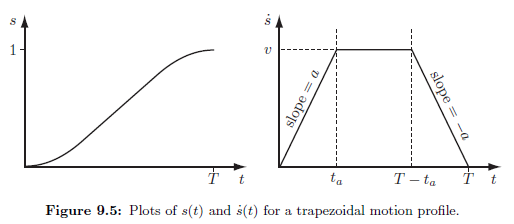
\includegraphics[width=0.7\linewidth]{Main/Chapter4/Images4/cap4_tray_9.png}
                \caption{Fotografía de un paraguas}
                \label{f:Cap4_tray_9}
            \end{figure}  
    
        La escala de tiempo trapezoidal no es tan suave como la escala de tiempo cúbico, pero tiene la ventaja, si se saben los límites constantes de las velocidades en las articulaciones  ${\dot{\theta}}_{limite} \in {\mathbb{R}}^n $   y los límites de aceleraciones de las articulaciones ${\ddot{\theta}}_{limite} \in {\mathbb{R}}^n $  , entonces el movimiento trapezoidal usado por la mayor $v$ y $a$  debe satisfacer:
        
        \begin{equation}
             \left| ({\theta}_{final}-{\theta}_{inicio})v \right|   \leq {\dot{\theta}}_{limite}
            \label{eq:cap4_tray_28}
        \end{equation}
        
        \begin{equation}
             \left| ({\theta}_{final}-{\theta}_{inicio})a \right|   \leq {\ddot{\theta}}_{limite}
            \label{eq:cap4_tray_29}
        \end{equation}
        
        Si ${v^2}/a > 1$, el robot nunca alcanza la velocidad $v$  durante el movimiento. El movimiento trifásico de aceleración-velocidad constante-desaceleración se convierte en un movimiento bifásico de aceleración-desaceleración llamado “bang-bang” y el perfil trapezoidal $\dot{s}̇(t)$ de la ilustracion \ref{f:Cap4_tray_9} se convierte en un triángulo.
        
        \begin{figure}[htb]
                \centering
                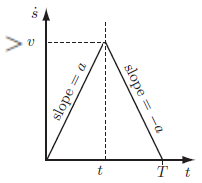
\includegraphics[width=0.27\linewidth]{Main/Chapter4/Images4/cap4_tray_10.png}
                \caption{Fotografía de un paraguas}
                \label{f:Cap4_tray_10}
            \end{figure} 
    
    
            \newpage

        Suponiendo que ${v^2}/a \leq 1$ , el movimiento trapezoidal está completamente especificado por $v$,$a$,$t_a$ y  $T$ ,pero solo dos de estos pueden especificarse independientemente ya que deben satisfacer $s(T)=1$  y $v=at_a$ . Es poco probable que se especifique  $t_a$  de forma independiente, por lo que se elimina de las ecuaciones de movimiento mediante la sustitución ${t}_{a}=v/a$ . El perfil de movimiento durante las tres etapas (aceleración, velocidad constante, desaceleración) se puede escribir en términos de $v$,$a$ y $T$ de la siguiente manera:
        
        Para $0 \leq t \leq \frac{v}{a}$ :
        \begin{equation}
            \ddot{s}(t)=a 
            \label{eq:cap4_tray_30}
        \end{equation}
        \begin{equation}
            \dot{s}(t)=at
            \label{eq:cap4_tray_31}
        \end{equation}
        \begin{equation}
             s(t)=\frac{1}{2}at^2
            \label{eq:cap4_tray_32}
        \end{equation}
        
        Para $ \frac{v}{a} \leq t \leq  (T-\frac{v}{a})$ :
        \begin{equation}
            \ddot{s}(t)=0 
            \label{eq:cap4_tray_33}
        \end{equation}
        \begin{equation}
            \dot{s}(t)=v
            \label{eq:cap4_tray_34}
        \end{equation}
        \begin{equation}
             s(t)=vt - \frac{v^2}{2a}
            \label{eq:cap4_tray_35}
        \end{equation}
        
        Para $ (T-\frac{v}{a}) \leq t \leq  T$ :
        \begin{equation}
            \ddot{s}(t)=-a 
            \label{eq:cap4_tray_36}
        \end{equation}
        \begin{equation}
            \dot{s}(t)=a(T-t)
            \label{eq:cap4_tray_37}
        \end{equation}
        \begin{equation}
             s(t)=\frac{2avT-2v^2-a^2(t-T)^2}{2a}
            \label{eq:cap4_tray_38}
        \end{equation}        
        
    Dado que solo dos de $v$, $a$ y $T$ pueden elegirse independientemente, se tiene 3 opciones:
    
    \begin{itemize}
        \item Se elige $v$ y $a$  tal que $v^2/a \leq 1$ , asegurando un perfil trapezoidal de tres etapas y se resuelve $s(T)=1$ para $T$:
        \begin{equation}
            T=\frac{a + v^2}{va}
            \label{eq:cap4_tray_39}
        \end{equation}
        Si $v$ y $a$  corresponden a las mayores velocidades y aceleraciones articulares posibles, este es el tiempo mínimo posible para el movimiento.
        
        \item 	Se elige $v$ y $T$ de modo que $2 \geq vT \geq 1$ , garantizando un perfil trapezoidal de tres etapas y que la velocidad máxima $v$ sea suficiente para alcanzar $s = 1$ en el tiempo $T$. Resolviendo $s(T)=1$   para $a$:
        \begin{equation}
            a=\frac{v^2}{vT-1}
            \label{eq:cap4_tray_40}
        \end{equation}
        
        \item 	Eligiendo $a$ y $T$ tal que $aT^2 \geq 4$ , asegurando que el movimiento sea completo en el tiempo $T$, resolviendo  $s(T)=1$  para $v$ : 
        \begin{equation}
            v=\frac{1}{2}(aT-\sqrt{a}\sqrt{aT^2 - 4})
            \label{eq:cap4_tray_41}
        \end{equation}
    \end{itemize}
        
    Esta misma representación del perfil trapezoidal en esta sección tambien se puede encontrar en el libro \cite{tray_trape}.
        
        
                \newpage
